% Options for packages loaded elsewhere
\PassOptionsToPackage{unicode}{hyperref}
\PassOptionsToPackage{hyphens}{url}
\PassOptionsToPackage{dvipsnames,svgnames*,x11names*}{xcolor}
%
\documentclass[
  12pt,
]{article}
\usepackage{lmodern}
\usepackage{amssymb,amsmath}
\usepackage{ifxetex,ifluatex}
\ifnum 0\ifxetex 1\fi\ifluatex 1\fi=0 % if pdftex
  \usepackage[T1]{fontenc}
  \usepackage[utf8]{inputenc}
  \usepackage{textcomp} % provide euro and other symbols
\else % if luatex or xetex
  \usepackage{unicode-math}
  \defaultfontfeatures{Scale=MatchLowercase}
  \defaultfontfeatures[\rmfamily]{Ligatures=TeX,Scale=1}
\fi
% Use upquote if available, for straight quotes in verbatim environments
\IfFileExists{upquote.sty}{\usepackage{upquote}}{}
\IfFileExists{microtype.sty}{% use microtype if available
  \usepackage[]{microtype}
  \UseMicrotypeSet[protrusion]{basicmath} % disable protrusion for tt fonts
}{}
\makeatletter
\@ifundefined{KOMAClassName}{% if non-KOMA class
  \IfFileExists{parskip.sty}{%
    \usepackage{parskip}
  }{% else
    \setlength{\parindent}{0pt}
    \setlength{\parskip}{6pt plus 2pt minus 1pt}}
}{% if KOMA class
  \KOMAoptions{parskip=half}}
\makeatother
\usepackage{xcolor}
\IfFileExists{xurl.sty}{\usepackage{xurl}}{} % add URL line breaks if available
\IfFileExists{bookmark.sty}{\usepackage{bookmark}}{\usepackage{hyperref}}
\hypersetup{
  pdftitle={Esqueleto do TF},
  pdfauthor={Henrique S Requejo},
  colorlinks=true,
  linkcolor=black,
  filecolor=Maroon,
  citecolor=Blue,
  urlcolor=blue,
  pdfcreator={LaTeX via pandoc}}
\urlstyle{same} % disable monospaced font for URLs
\usepackage[margin=1in]{geometry}
\usepackage{graphicx,grffile}
\makeatletter
\def\maxwidth{\ifdim\Gin@nat@width>\linewidth\linewidth\else\Gin@nat@width\fi}
\def\maxheight{\ifdim\Gin@nat@height>\textheight\textheight\else\Gin@nat@height\fi}
\makeatother
% Scale images if necessary, so that they will not overflow the page
% margins by default, and it is still possible to overwrite the defaults
% using explicit options in \includegraphics[width, height, ...]{}
\setkeys{Gin}{width=\maxwidth,height=\maxheight,keepaspectratio}
% Set default figure placement to htbp
\makeatletter
\def\fps@figure{htbp}
\makeatother
\setlength{\emergencystretch}{3em} % prevent overfull lines
\providecommand{\tightlist}{%
  \setlength{\itemsep}{0pt}\setlength{\parskip}{0pt}}
\setcounter{secnumdepth}{5}
\usepackage[utf8]{inputenc}
\usepackage{subfig}
\usepackage{float}
\usepackage{amsbsy}
\usepackage[portuguese]{babel}

\usepackage{booktabs}
\usepackage{longtable}
\usepackage{array}
\usepackage{multirow}
\usepackage{wrapfig}
\usepackage{float}
\usepackage{colortbl}
\usepackage{pdflscape}
\usepackage{tabu}
\usepackage{threeparttable}
\usepackage{threeparttablex}
\usepackage[normalem]{ulem}
\usepackage{makecell}
\usepackage{xcolor}
\usepackage{setspace}
\usepackage{indentfirst}
\usepackage[font=small,labelfont=bf]{caption}

\newcommand*{\secref}[1]{Section~\ref{#1}}

\floatplacement{figure}{H}
\onehalfspacing
\graphicspath{ {./images/} }
\setlength{\parindent}{2em}
\AtBeginDocument{\let\maketitle\relax}
\usepackage{booktabs}
\usepackage{longtable}
\usepackage{array}
\usepackage{multirow}
\usepackage{wrapfig}
\usepackage{float}
\usepackage{colortbl}
\usepackage{pdflscape}
\usepackage{tabu}
\usepackage{threeparttable}
\usepackage{threeparttablex}
\usepackage[normalem]{ulem}
\usepackage{makecell}

\title{Esqueleto do TF}
\author{Henrique S Requejo}
\date{16/11/2020}

\begin{document}
\maketitle

\pagenumbering{gobble}

\thispagestyle{empty}
\begin{center}
    \vspace*{1cm}
    \textbf{\textsc{Universidade de São Paulo\\Campus Butantã\\Instituto de Matemática e Estatística}}\\

    
    \vskip 4cm
    \textsc{\Large{Um teste do algoritmo de modularidade Louvain como uma ferramenta para detectar espécies-chave em redes de interações multicamada}}
    
    \vskip 4cm
    {\large{Aluno: Henrique Suzuki Requejo\\
    Orientador: Prof. Dr. Marco A. R. Mello \\
    Curso: Matemática Aplicada e Computacional\\
    Habilitação: Ciências Biológicas\\}}
    
    \vskip 4cm
    \normalsize{São Paulo, 2021}
\end{center}

\newpage
\thispagestyle{empty}
    \begin{center}
        \vspace*{2.3 cm}
        \textbf{\Large{Um teste do algoritmo de modularidade Louvain como uma ferramenta para detectar espécies-chave em redes de interações multicamada}}\\
        \vspace*{2 cm}
    \end{center}

    \vskip 2cm

    \begin{flushright}
    Trabalho de Conclusão de Curso submetido \\ à Universidade de São Paulo, como requisito \\ necessário para obtenção do grau de Bacharel \\ em Matemática Aplicada e Computacional
    \end{flushright}
 \vskip 6cm
 \begin{center}
    São Paulo, 2021
 \end{center}
\pagebreak

\pagebreak

\tableofcontents

\pagebreak

\pagenumbering{arabic}

\hypertarget{resumo}{%
\section{Resumo}\label{resumo}}

Análises de modularidade oriundas da ciência de redes têm sido usadas na
Ecologia para operacionalizar conceitos como guilda, grupo funcional e
papel funcional. Contudo, essas análises têm sido feitas apenas para
redes monocamada, ou seja, que contém só um tipo de interação, portanto,
apenas uma classe de arestas. No caso do algoritmo de modularidade
Louvain, uma das grandes diferenças entre a tradicional versão
monocamada e a nova versão multicamada é a constante de acoplamento.
Essa constante, implementada no algoritmo multicamada, torna possível
que um mesmo nó pertença a dois módulos diferentes em camadas
diferentes. Neste projeto, queremos identificar os nós que resistem ao
aumento dessa força de acoplamento entre camadas, permanecendo em mais
de um módulo em diferentes camadas ao aumentarmos essa força de
acoplamento. Em redes de interações ecológicas, esses nós resistentes
devem representar espécies que desempenham papéis funcionais
importantes. Por exemplo, animais que são importantes tanto para a
polinização, quanto para a dispersão de sementes de duas ou mais
famílias de plantas. Para classificar as espécies com relação a sua
importância, comparamos a curva do número de módulos aos quais cada nó
pertence em função da variação na constante de acoplamento e do
parâmetro de resolução. Assim, selecionaremos os nós que apresentam
menor decaimento de módulos, ou seja, que permanecem um mais de um
módulo mesmo com força de acoplamento entre camadas, considerando
diferentes cenários de resolução. Até o momento foram analisadas as
redes de interações entre morcegos e plantas e de formigas e plantas. A
próxima etapa é avaliar se ganhamos informação relevante, tanto no nível
do nó como no nível dos módulos, na abordagem multicamada em comparação
à monocamada. Em seguida, repetiremos essas mesmas análises para redes
sintéticas, dessa maneira, poderemos verificar se o método é eficaz em
várias redes diferentes. Isso nos permitirá entender melhor o que faz as
espécies que eles representam serem mais importantes do que outras para
manter funções e serviços ecossistêmicos vitais.

\pagebreak

\hypertarget{modularidade-de-newman-e-girvan}{%
\section{Modularidade de Newman e
Girvan}\label{modularidade-de-newman-e-girvan}}

A ciência de redes tem sido usada para investigar sistemas ecológicos
desde o século XIX (Ings \& Hawes, 2018). Dentre vários avanços, essa
abordagem nos permitiu entender melhor como várias espécies afetam umas
às outras por meio de interações diretas e indiretas. Esse entendimento
levou a importantes insights sobre a estrutura, função e dinâmica de
redes de interações (Pilosof et al., 2017).

Uma forma de obtermos estes insights é olhar para a estrutura de módulos
da rede, o que pode revelar alguns padrões escondidos em meio à
complexidade de nós e conexões. Estes módulos são compostos por nós mais
conectados entre si do que com outros nós de fora do módulo. A
capacidade de encontrar e analisar esses módulos pode fornecer ajuda
inestimável para entender mais a fundo a estrutura das redes (Newman \&
Girvan, 2004).

É relativamente fácil identificar módulos em redes pequenas e pouco
conectadas. Porém, essa tarefa se torna muito difícil quando analisamos
redes mais complexas, com milhares, ou até mesmo milhões, de nós
distribuídos em várias camadas. Então, como podemos identificar módulos
em redes complexas? Existem muitas formas, como por exemplo métodos
aglomerativos, divisivos, baseados em cliques e de otimização de
modularidade. Neste projeto vamos focar na otimização de modularidade.

Para otimizarmos a modularidade, precisamos de uma métrica que indique
se uma específica divisão da rede em módulos é melhor do que outra, para
então buscar qual seria a melhor divisão de módulos possível. Uma
métrica para medir a qualidade da modularidade de redes foi definida
pela primeira vez por Newman e Girvan (Newman \& Girvan, 2004) como:

\begin{equation} \label{eq:mod_basica}
    Q = \sum^{k}_{i=1}(e_{ii}-a^2_i)
\end{equation}

Onde \(e_{ii}\) representa a fração das conexões observadas dentro do
módulo \(i\) em relação ao total de conexões dentro da rede e \(a^2_i\)
representa a quantidade esperada de conexões no módulo \(i\).

Para determinar a proporção de conexões dentro dos módulos, suponha que
temos uma uma possível divisão de módulos dentro da rede representada
pela matriz de adjacência \(A_{ij}\), seja \(C_i\) o módulo que o nó
\(i\) está contido, então, a fração de conexões que conectam os vértices
que estão dentro de um mesmo módulo é:

\begin{equation} \label{eq:fracao_conect}
    \frac{\sum_{ij} A_{ij} \delta (c_i, c_j)}{\sum_{ij} A_{ij}} = \frac{1}{2m} \sum_{ij} A_{ij} \delta (c_i, c_j) 
\end{equation}

Onde \(\delta\) é o delta de kronecker, que retorna o valor 1 caso
\(c_i = c_j\) e zero caso contrário; a variável \(m\) representa o
número total de conexões da rede. Falta agora definirmos uma forma de
medir a quantidade esperada de nós dentro do módulo. Se conectarmos os
vértices de forma aleatória, preservando os graus de cada nó,
representados pela variável \(k\), temos que a probabilidade de existir
uma conexão entre os nós \(i\) e \(j\) é \(k_i k_j / 2m\) . Dessa forma,
temos que a modularidade descrita acima pode ser reescrita de uma forma
mais operacional (Blondel et al., 2008) como:

\begin{equation} \label{eq:blondel}
    Q = \frac{1}{2m} \sum_{ij} (A_{ij} - \frac{k_i k_j}{2m}) \delta(c_i c_j)
\end{equation}

Os valores da modularidade descrita acima podem variar entre zero e 1.

\pagebreak

\hypertarget{muxe9todo-louvain-para-otimizauxe7uxe3o-de-modularidade}{%
\section{Método Louvain para otimização de
modularidade}\label{muxe9todo-louvain-para-otimizauxe7uxe3o-de-modularidade}}

Se dividirmos a rede em módulos e o valor de modularidade definido por
Newman e Girvan for alto, temos que a divisão de módulos escolhida é
boa. Dessa forma, basta dividirmos a rede em diferentes módulos visando
maximizar o valor da modularidade Newman-Girvan. Porém, esta não é uma
tarefa fácil, já que a otimização de modularidade é um problema
NP-difícil (Brandes et al., 2008). Um problema NP (Non Deterministic
Polynomial Time) é um problema que leva um tempo exponencial para ser
resolvido, por exemplo \(O(2^N)\). Estes problemas NP demoram muito para
serem computados, por exemplo, caso o problema possua uma complexidade
exponencial \(O(2^N)\) e \(N\) (tamanho da entrada) seja igual a 100, o
programa demoraria um tempo maior que a idade do universo para ser
resolvido. Um problema NP-difícil é um problema que é ao menos tão
difícil quanto um problema NP-completo.

Esta dificuldade computacional em dividir redes em módulos
significativos motivou a procura por métodos heurísticos para encontrar
agrupamentos que apresentam um alto valor de modularidade com uma
complexidade razoável. Este é o caso do método Louvain (Blondel et al.,
2008), que parece funcionar em um tempo \(O(M)\), onde \(M\) representa
o número total de conexões da rede, ou seja, é resolvido em tempo
polinomial, neste caso, linear com relação ao número de nós da rede.
Essa complexidade computacional permite que redes de grande escala
possam ser analisadas em tempo razoável, além de ser simples e de fácil
implementação.

A implementação do algoritmo Louvain consiste de dois passos básicos,
descritos em detalhe por Blondel et al. (2008). O primeiro passo agrupa
os nós em módulos de forma individual, favorecendo otimizações locais de
modularidade. O segundo passo transforma a rede original em uma nova
rede simplificada, cujo os novos nós são os módulos do passo anterior.
As conexões entre estes novos nós correspondem à soma das conexões entre
os módulos e cada nó agora tem um laço (conexão que liga um nó a ele
mesmo) cujo o peso é a soma das conexões dentro do módulo
correspondente. Esses dois passos são repetidos até que não exista mais
aumento no valor da modularidade. A figura \ref{fig:algoritmo_Louvain}
ilustra o algoritmo.

\begin{figure}[H] 
\centering
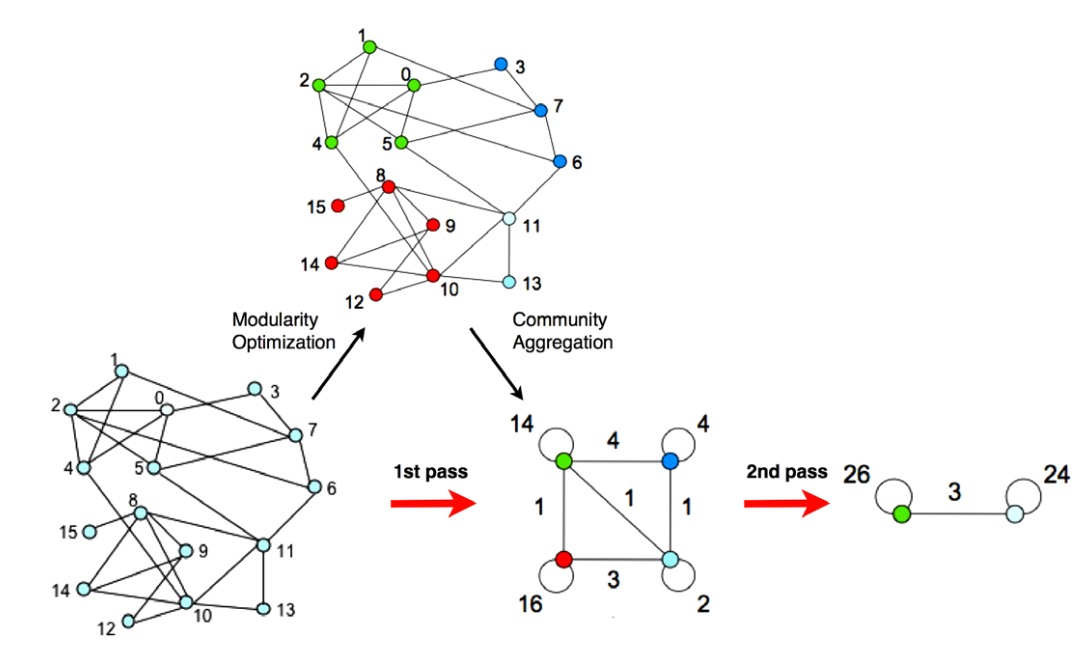
\includegraphics[width=0.8\textwidth]{./Figuras/Algoritmo_Louvain.png}
\caption{Extraído de Blondel et al. (2008). Visualização dos passos do algoritmo Louvain. Cada passo é feito em duas fases: uma onde a modularidade é otimizada permitindo somente mudanças locais de módulo e uma onde os módulos encontradas são agregadas e uma nova rede de módulos é construída.}
\label{fig:algoritmo_Louvain}
\end{figure}

Apesar deste ser um algoritmo ganancioso, ele apresenta boa detecção de
módulos que possuem sentido quando aplicados em redes reais (Blondel et
al., 2008; Meunier, 2009; Zhang et al., 2010) e é mais rápido que outros
algoritmos similares, como mostrado na tabela \ref{tab:tabela_blondel},
extraída de Blondel et al. (2008). Outra vantagem do método é que não
precisamos saber previamente o número de módulos que a rede deve ser
dividida.

\begin{table}[h!]
  \caption{Extraído de Blondel et al. (2008). Comparação entre os tempos computacionais dos algoritmos Clauset et al (CNM), Pons e Latapy (PL), Wakita e Tsurumi (WT) e Louvain (LV). Os resultados mostram a modularidade obtida e o tempo computacional para cada rede/método. Células em branco representam tempos computacionais maiores que 24 horas.}
  \label{tab:tabela_blondel}
  \centering
  \resizebox{\textwidth}{!}{ 
\begin{tabular}{ | c | c | c | c | c | c | c | c | }
\hline
     & \textbf{Karate} & \textbf{Arxiv} & \textbf{Internet} & \textbf{Web nd.edu} & \textbf{Telefone} & \textbf{Web uk2005} & \textbf{WebBase 2001} \\ \hline
    Nós / Conexões & 34/77 & 9k/24k & 70k/351k & 325k/1M & 2.04M/5.4M & 39M/783M & 118M/1B \\ \hline
    CNM & 0.38/0s & 0.772/3.6s & 0.692/799s & 0.927/5034s & - & - & - \\ \hline
    PL & 0.42/0s & 0.752/3.3s & 0.729/575s & 0.895/6666s & - & - & - \\ \hline
    WT & 0.42/0s & 0.761/0.7s & 0.667/62s & 0.898/248s & 0.553/367s & - & - \\ \hline
    LV & 0.42/0s & 0.813/0s & 0.781/1s & 0.935/3s & 0.76/44s & 0.935/3s & 0.984/152min \\ \hline
\end{tabular}
}
\end{table}

Por outro lado, o método Louvain também apresenta limitações (Good et
al., 2010). Dentre as mais expressivas estão o limite de resolução, o
problema de degeneração e o fato de o algoritmo não ser determinístico.
O problema de limite de resolução ocorre pois o algoritmo pode não parar
nos módulos ``intuitivos'' devido a uma segunda passagem pela
modificação dos módulos. Já o problema de degeneração ocorre pois podem
existir muitas soluções com valor de modularidade próximos do máximo
global, nesses casos é muito difícil encontrar o máximo global e de
realmente afirmar se o máximo global possui significância científica
maior que os máximos locais com valores de modularidade similares.

Uma característica interessante do método é que não é possível, pela
própria natureza do algoritmo, que um mesmo nó esteja presente em
diferentes módulos, essa sobreposição de módulos é chamada dentro da
área de modularidade de redes de \textit{overlapping communities}.
Porém, ao adaptarmos a forma de calcular a modularidade para multicamada
(Mucha et al., 2010), existe a possibilidade de que um mesmo nó pertença
a diferentes módulos em diferentes camadas ao ajustarmos um parâmetro de
entrada. Esta diferença é interessante e será usada para tentar
encontrar espécies-chave que são boas conectoras entre grupos diferentes
em camadas diferentes.

\pagebreak

\hypertarget{modularidade-multicamada}{%
\section{Modularidade Multicamada}\label{modularidade-multicamada}}

Apesar do amplo estudo de redes para compreensão de sistemas e tomada de
decisão, estas redes são normalmente estudadas de forma desconexa de
outras redes ou então agregando-se várias redes em uma única rede
(Pilosof et al., 2017). Uma maneira de aumentarmos as informações usadas
no estudo de redes é usar redes multicamada (Pilosof et al., 2017).
Quando usadas para representar sistemas ecológicos, as redes multicamada
podem ter suas camadas definidas através de interações de diferentes
tipos, ou que acontecem em diferentes localidades ou estações do ano,
por exemplo (Pilosof et al., 2017).

No caso deste projeto, a rede em foco é a rede multicamada onde as
camadas são definidas pelo tipo de interação, ou seja, todos os nós
estão presentes em todas as camadas e apenas o tipo de ligação
(interações) entre os nós é o que muda em cada camada. Assim, nesse tipo
de rede há duas classes maiores de arestas: intracamada, que conecta nós
dentro de uma camada, e intercamada, que conecta um mesmo nó entre duas
camadas. Este tipo de rede é chamada de \textit{multiplex} (Mucha et
al., 2010), que é uma subdivisão da grande categoria definida como redes
multicamada.

Redes multiplex também podem ter sua modularidade analisada pelo método
Louvain (Mucha et al., 2010). Essa adaptação consiste basicamente na
mudança da forma como a função da modularidade é calculada, incluindo um
parâmetro \(\omega\) que controla o acoplamento entre as diferentes
camadas da rede. Há também o parâmetro de resolução \(\omega\), que pode
enviesar a tendência do algoritmo em encontrar módulos de escalas
menores ou maiores. A generalização da equação de modularidade (Mucha et
al., 2010) é dada por:

\begin{equation} \label{eq:1}
Q^{M} = \frac{1}{\mu} \sum_{ij\alpha\beta} \left[ \left(A_{i\alpha,j\alpha} - \gamma_{\alpha} \frac{k_{i\alpha} k_{j\alpha}}{2m_\alpha} \right) \delta_{\alpha,\beta} + \omega A_{i\alpha,j\beta} \delta_{ij} \right] \delta(c_{i\alpha}, c_{j \beta})
\end{equation}

Onde \(\delta\) é o delta de kronecker, que retorna o valor 1 caso
\(c_{i\alpha} = c_{j \beta}\) e zero caso contrário; a variável \(m\)
representa a soma de do grau de cada nó na camada \(\alpha\);
\(A_{i\alpha,j\alpha}\) é a matriz de adjacência na camada \(\alpha\);
\(A_{i\alpha,j\beta}\) é a matriz de adjacência entre camadas;
\(k_{i\alpha}\) representa o grau do nó \(i\) na camada \(\alpha\) e
\(\mu = \sum_{i,j, \alpha}A_{i\alpha,j\alpha} + \omega \sum_{i,\alpha,\beta} A_{i\alpha,j\beta}\).
Note que se utilizarmos \(\omega = 0\) e \(\gamma = 1\), a equação de
modularidade generalizada (eq. \ref{eq:1}) é proporcional a média da
modularidade monocamada (Newman, 2004; Newman \& Girvan, 2004) de cada
camada. Isto também está descrito em Bianconi (2018), pg. 147-148:

\begin{equation} \label{eq:2}
Q^{M} = \frac{1}{\mu} \sum_{\alpha} \frac{1}{2m_\alpha} \sum_{ij} \left(A_{i\alpha,j\alpha} - \gamma_{\alpha} \frac{k_{i\alpha} k_{j\alpha}}{2m_\alpha} \right) \delta(c_{i\alpha}, c_{j\alpha}) \end{equation}

\hypertarget{paruxe2metros-de-acoplamento-omega-e-resoluuxe7uxe3o-gamma-na-pruxe1tica}{%
\section{\texorpdfstring{Parâmetros de acoplamento (\(\omega\)) e
resolução (\(\gamma\)) na
prática}{Parâmetros de acoplamento (\textbackslash omega) e resolução (\textbackslash gamma) na prática}}\label{paruxe2metros-de-acoplamento-omega-e-resoluuxe7uxe3o-gamma-na-pruxe1tica}}

Como a escolha dos parâmetros de resolução e acoplamento é arbitrária,
ficam as perguntas: qual seria o melhor valor para aplicar em uma dada
rede? Existe apenas um único valor adequado ou o valor a ser escolhido
depende do da pergunta que pretendo responder? Quais são os efeitos na
prática quando variamos \(\gamma\) e \(\omega\)? Com o objetivo de
responder essas perguntas e auxiliar outros cientistas na escolha dos
valores de \(\gamma\) e \(\omega\), vamos analisar essas questões em
detalhes.

O parâmetro \(\omega\) está contido no intervalo (0,1).Zero (0)
representa o desacoplamento total das camadas (cada camada é tratada
como uma rede individual) e a modularidade final é a média da
modularidade de cada camada. Um (1) representa o acoplamento máximo, que
faz com que a rede multiplex se comporte como uma rede monocamada. Na
prática, isso significa que, quando aumentamos os valores da constante
de acoplamento \(\omega\), aumentamos o peso das arestas intercamada
(Mucha et al., 2010), isso faz com que as camadas tenham maior
influência umas sobre as outras, favorecendo a formação de módulos
multicamada. Quando diminuímos \(\omega\), o contrário ocorre, o que
favorece a formação de módulos monocamada.

O parâmetro de resolução foi introduzido por Reichardt \& Bornholdt
(2006) para avaliar redes monocamada e depois estendido para a
modularidade generalizada multicamada (Mucha et al., 2010). De uma forma
geral, se \(\gamma_2 > \gamma_1\), os módulos encontrados com
\(\gamma_2\) possuem menos nós (módulos menores) e são mais numerosos
(maior quantidade de módulos). Os módulos encontrados com \(\gamma_2\)
podem ser submódulos dos obtidos usando \(\gamma_1\), mas nem sempre é o
caso (Reichardt \& Bornholdt, 2006). Lembrando que
\(0 \leq \gamma \leq \infty\). Porém, não faz sentido aumentarmos
\(\gamma\) para valores muito altos, já que existe um limite a partir do
qual os módulos se tornam tão pequenos que cada módulo passa a ter
apenas um nó.

Vamos usar a rede multiplex Famílias de Florença (Kent, 1978) para
ilustrar graficamente o que ocorre quando variamos os parâmetros
\(\omega\) e \(\gamma\). Essa rede foi escolhida por ser pequena, o que
facilita sua visualização. A figura \ref{fig:Mosaico1} mostra a
distribuição dos módulos sobre as duas camadas da rede para diferentes
valores de \(\omega\) e \(\gamma\).

\begin{figure}[h!]
    \centering
    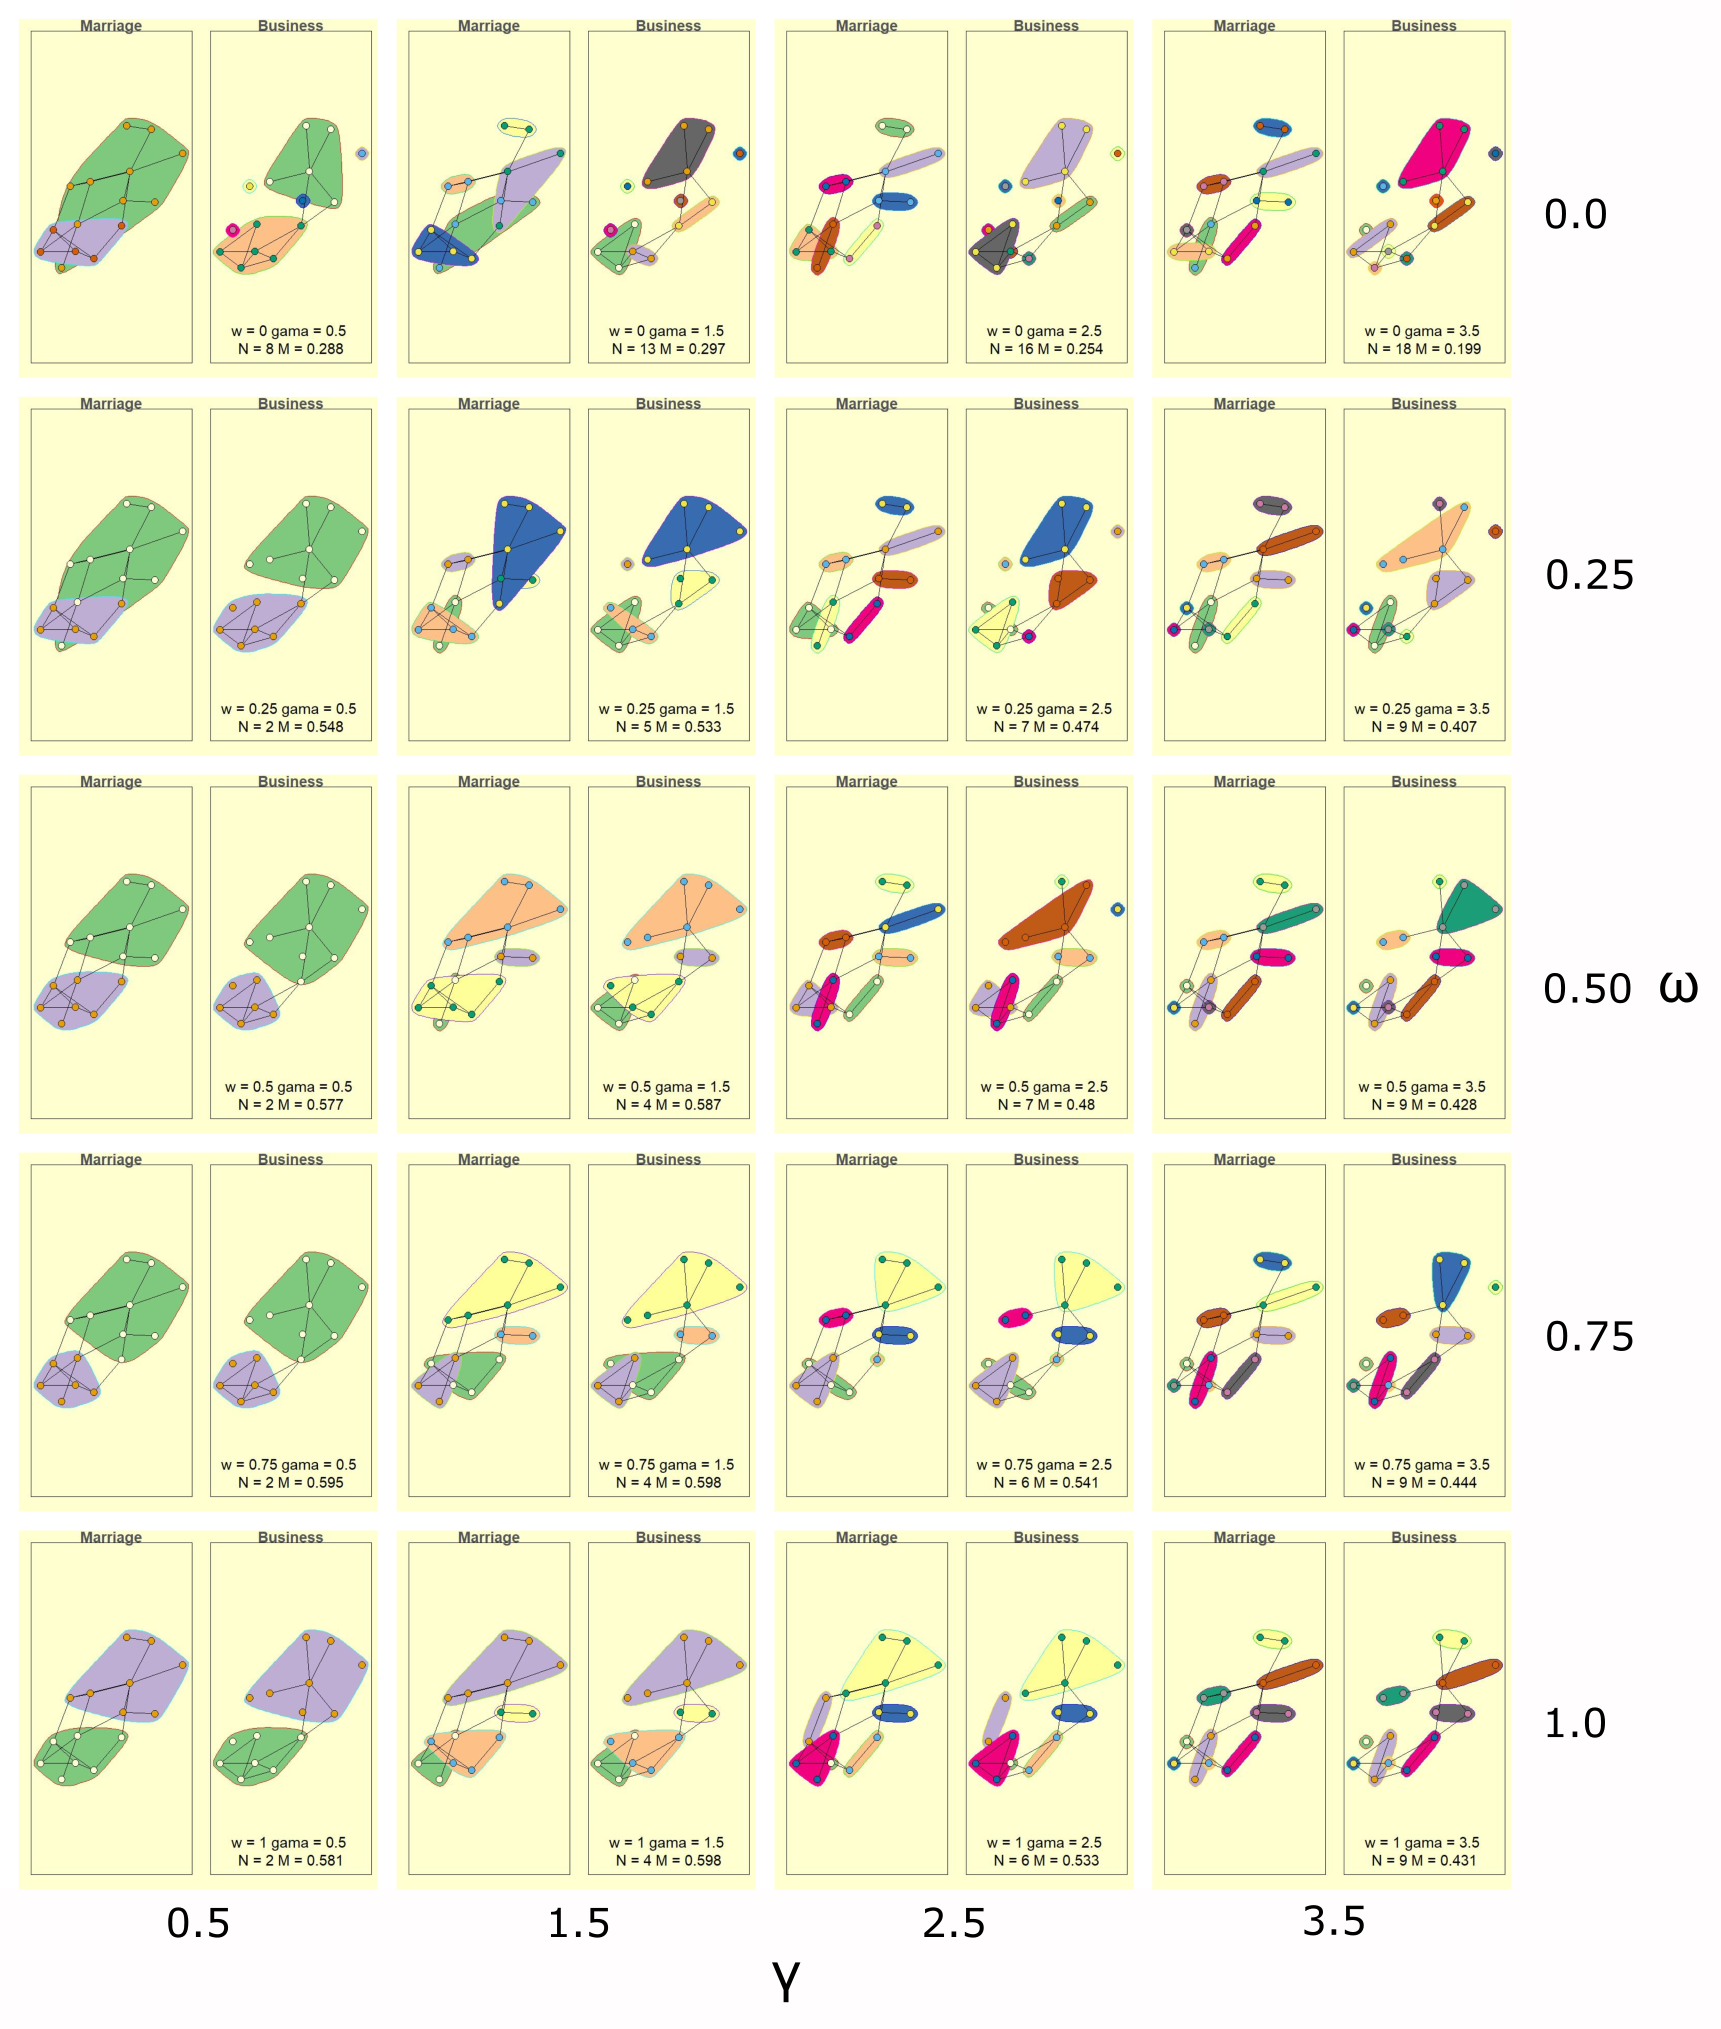
\includegraphics[width=1\textwidth]{./Figuras/Mosaico_edit.png}
    \caption{Módulos formados usando diferentes valores de acoplamento $\omega$ e resolução $\gamma$. Valores de $\omega$ variam no eixo y e valores de $\gamma$ variam no eixo x.}
    \label{fig:Mosaico1}
\end{figure}

\pagebreak

Quanto maiores o os valores de \(\gamma\) e menores os valores de
\(\omega\), menores e mais numerosos são os módulos e vice-versa. A
figura \ref{fig:Mosaico2} mostra o número de módulos para a rede exemplo
Famílias de Florença, onde podemos ver que ocorre o previsto na teoria.

\begin{figure}[h!]
    \centering
    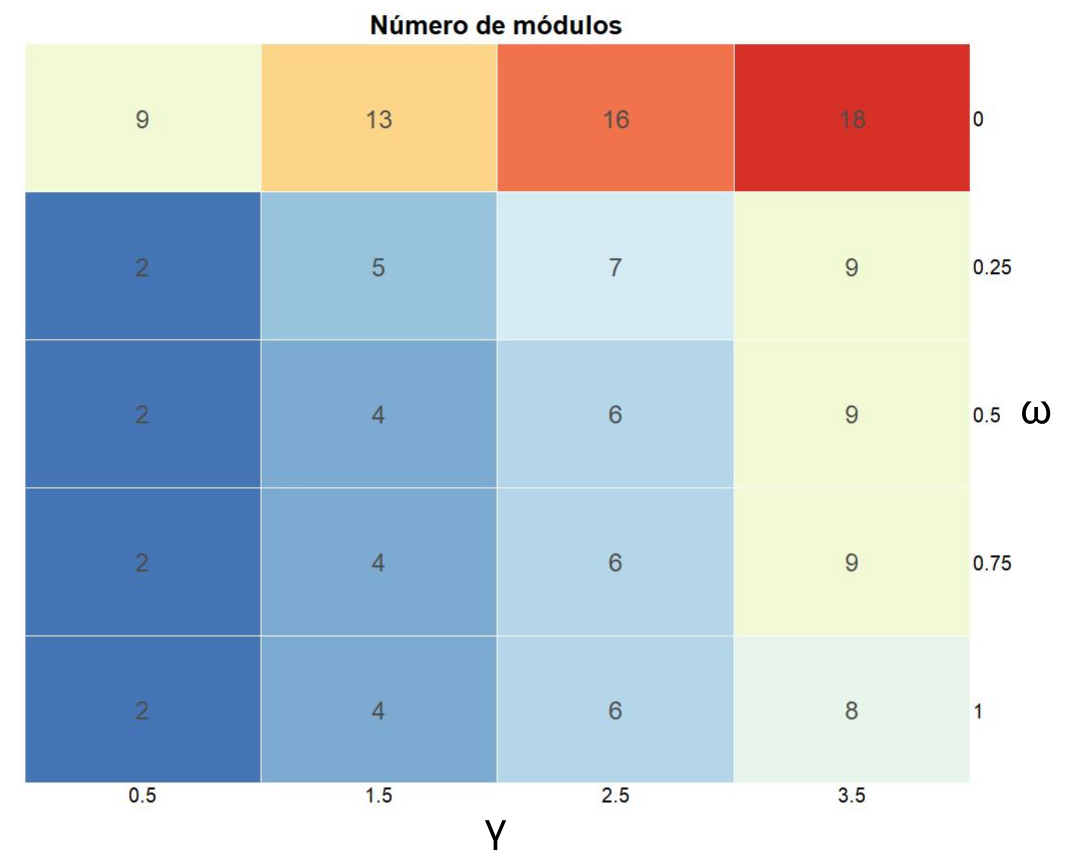
\includegraphics[width=1\textwidth]{./Figuras/Mosaico_numero_de_modulos_edit.png}
    \caption{Número de módulos totais da rede para diferentes valores de acoplamento $\omega$ e resolução $\gamma$. Valores de $\omega$ variam no eixo y e valores de $\gamma$ variam no eixo x.}
    \label{fig:Mosaico2}
\end{figure}

\pagebreak

Mas, afinal, quais valores devo escolher para esses dois parâmetros? A
resposta mais correta é: depende. Depende de qual propriedade da rede
queremos enfocar e qual pergunta queremos responder com esse enfoque.
Por exemplo, se quisermos verificar quais são os ``grandes módulos'' da
rede, devemos usar um valor de \(\gamma\) mais baixo, mas se quisermos
olhar para os módulos menores (mais ``íntimos'') ou submódulos dos
``grandes módulos'' obtidos com um \(\gamma\) mais baixo, um \(\gamma\)
maior seria mais indicado.

Se quisermos que as conexões de uma camada influenciem mais a outra
camada, devemos usar um \(\omega\) mais alto, coso contrário, melhor
usar um \(\omega\) mais baixo. Vamos usar agora como exemplo aa
redemorcego-planta (Mello et al., 2019), onde existem duas camadas: uma
de nectarívoria e outra de frugivoria. Se quisermos encontrar módulos
onde existam morcegos com dietas mais similares entre si, um \(\omega\)
mais alto é recomendado, pois a frugivoria e a nectarivoria ficaram com
alta influência uma sobre a outra no cálculo dos módulos. Já se
quisermos separar os morcegos com uma preferência maior por flores, por
frutos ou que tenham uma dieta equilibrada, podemos usar um \(\omega\)
menor, porque assim aumenta a tendência dos módulos se formarem pesando
mais as interações dentro de cada camada da rede. IIsso faz com que os
morcegos estejam em grupos que priorizam mais a nectarivoria ou a
frugivoria ou até mesmo que possuem interações equilibradas entre
camadas (estão em dois grupos em camadas diferentes).

Interpretação, conhecimento específico da área que a rede representa e
saber o que queremos enxergar são os fatores principais para a escolha
dos valores de \(\omega\) e \(\gamma\)

Caso quisermos apenas obter uma distribuição de módulos confiável sem a
necessidade de interpretação, podemos escolher um valor de \(\omega\) e
\(\gamma\) que maximiza a modularidade. Os valores de \(\omega\) e
\(\gamma\) que maximizam a modularidade diferem para cada rede. A figura
\ref{fig:Mosaico3} mostra os valores da modularidade para diferentes
valores de \(\omega\) e \(\gamma\) da rede exemplo Famílias de Florença.

\begin{figure}[h!]
    \centering
    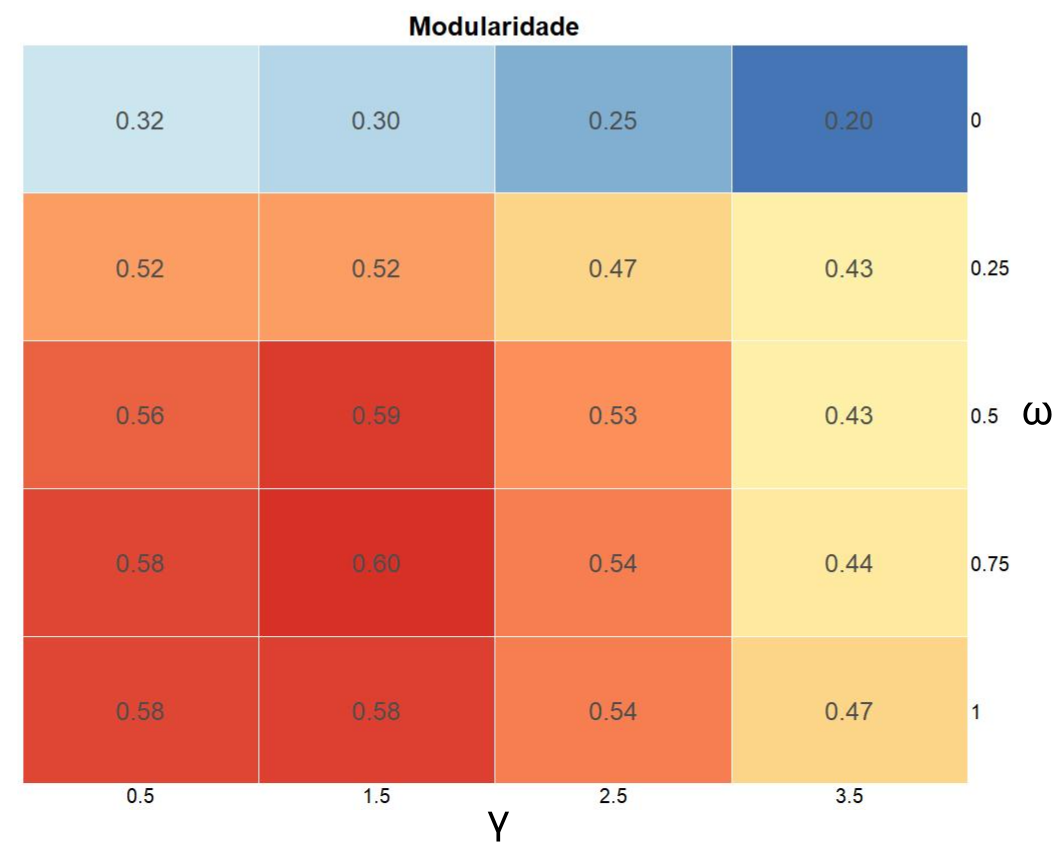
\includegraphics[width=1\textwidth]{./Figuras/Mosaico_modularidade_edit.png}
    \caption{Valor da modularidade para diferentes valores de acoplamento $\omega$ e resolução $\gamma$. Valores de $\omega$ variam no eixo y e valores de $\gamma$ variam no eixo x.}
    \label{fig:Mosaico3}
\end{figure}

Com a resolução do ensaio feito, os valores mais indicados para a rede
famílias de florença seriam \(\omega = 0.75\) e \(\gamma = 1.5\). Para
valores mais precisos, basta aumentar as partições de \(\gamma\) e
\(\omega\) ou refinar os valores de \(\gamma\) e \(\omega\) em torno dos
máximos obtidos no ensaio anterior.

Também existe a possibilidade de que os valores de modularidade fiquem
muito próximos uns dos outros. Nesse caso, é comum que os módulos fiquem
muito similares entre si, então, é possível escolher qualquer um dos
valores de \(\omega\) e \(\gamma\). Caso os módulos fiquem muito
diferentes entre si (um caso mais raro), uma interpretação de um
especialista na área que a rede está retratando é fundamental.

\clearpage

\hypertarget{variuxe1vel-g-e-g_norm}{%
\section{\texorpdfstring{Variável \(G\) e
\(G_{norm}\)}{Variável G e G\_\{norm\}}}\label{variuxe1vel-g-e-g_norm}}

\hypertarget{variuxe1vel-g}{%
\subsection{Variável G}\label{variuxe1vel-g}}

A variável G representa o número de módulos que um determinado nó
pertence. Como o algoritmo Louvain não permite que um mesmo nó participe
de mais de um módulo dentro de uma mesma camada, G é uma variável
discreta inteira que possui o mínimo de 1 e o máximo igual ao número de
camadas da rede estudada. G possui valores bem definidos nos extremos,
se \(\omega = 0 \Rightarrow G = 1\) e se
\(\omega = 0 \Rightarrow G = \text{ número total de camadas da rede}\).
Entre estes valores de \(\omega\) o comportamento de G é variado, mas
tende a cair conforme a força de acoplamento \(\omega\) aumenta. O
comportamento do decaimento de G em relação a \(\omega\) é diferente
para cada nó da rede, alguns nós resistem e permanecem em mais de um
módulo ao aumentarmos \(\omega\), já outros rapidamente passam a
pertencer a apenas um módulo ao aumentarmos \(\omega\). A figura
\ref{fig:Figura_G} ilustra o comportamento de diferentes nós ao
aumentarmos \(\omega\). A figura \ref{fig:Exemplo_decai} mostra um
exemplo de curva de decaimento de G em relação a \(\omega\).

\begin{figure}[H] 
\centering
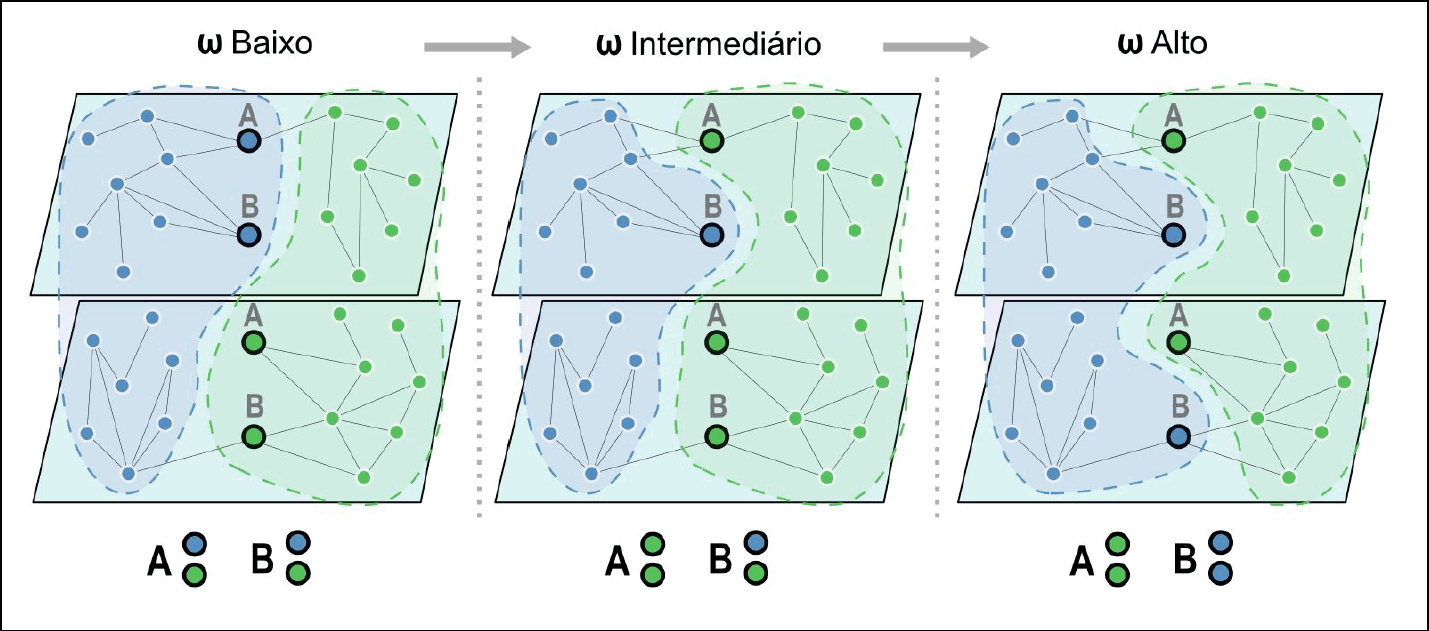
\includegraphics[width=0.8\textwidth]{./Figuras/Figura_G.png}
\caption{Esquema ilustrativo do que ocorre com alguns nós ao aumentarmos o parâmetro $\omega$. Para valores de $\omega$ baixos, vemos que os nós A e B estão em módulos diferentes em camadas diferentes. Ao aumentarmos a força de acoplamento $\omega$, o nó A passa a pertencer ao módulo verde tanto na camada superior como na camada inferior, já o nó B resiste e permanece no módulo azul na camada superior e no módulo verde na camada inferior. Se aumentarmos ainda mais a força de acoplamento $\omega$, em algum momento o nó B acaba cedendo e passa a pertencer a apenas um módulo nas duas camadas.}
\label{fig:Figura_G}
\end{figure}

\begin{figure}[H] 
\centering
\setlength{\fboxsep}{0pt}%
\setlength{\fboxrule}{0.25pt}%
\fbox{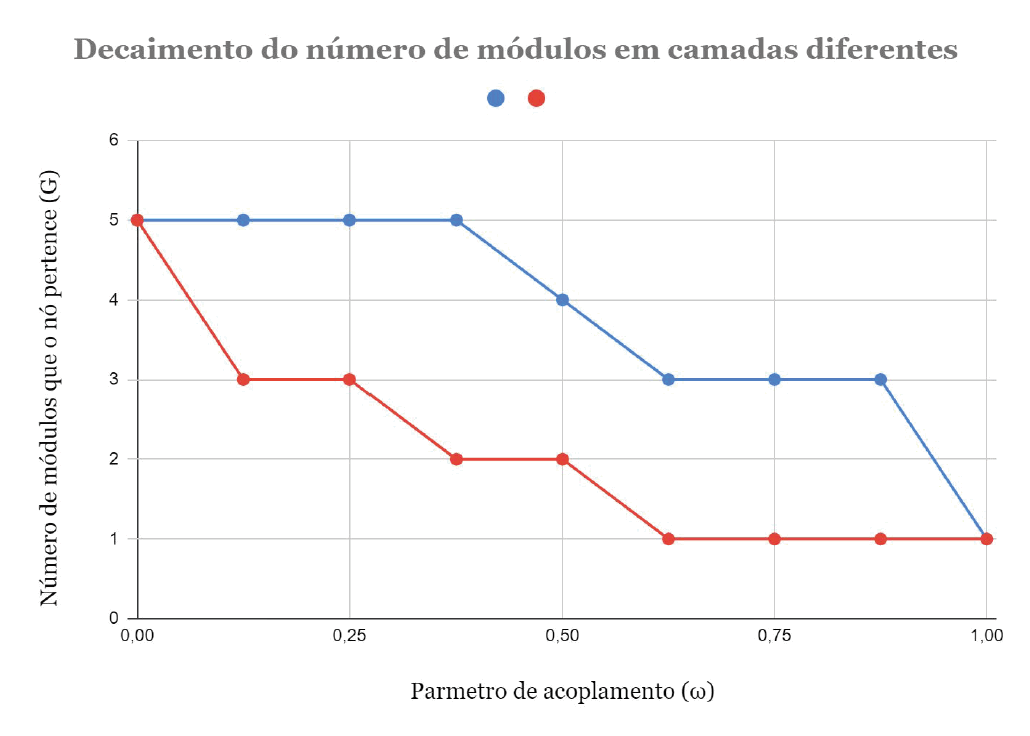
\includegraphics[width=0.7\textwidth]{./Figuras/Exemplo_decai.png}}
\caption{Exemplo hipotético de decaimentos de G (módulos que o nó pertence em diferentes camadas) em relação ao parâmetro $\omega$ (constante de acoplamento) esperados. O nó representado pela cor vermelha possui um decaimento rápido de G, portanto, representa uma espécie pouco conectiva do ponto de vista da rede multicamada como um todo. O contrário ocorre com a espécie representada pelo nó azul.}
\label{fig:Exemplo_decai}
\end{figure}

Como o algoritmo Louvain não é determinístico (pode retornar diferentes
resultados a cada compilação) e a variável G é inteira e discreta, para
termos uma maior confiabilidade precisamos repetir o processo várias
vezes para cada valor de \(\omega\) e extrair uma média de G para cada
nó. Assim o valor médio de G é dado por:

\begin{equation} \label{eq:3}
    \overline{G_{\omega}} = \frac{1}{I} \sum_{i=1}^{I} G_{i}
\end{equation}

Onde \(I\) se refere ao número de iterações.

Repetindo isso para diferentes valores de \(\omega\), teremos uma curva
de decaimento \(\overline{G}\) por \(\omega\).

Podemos agora repetir esse processo para diferentes valores de
\(\gamma\), assim vamos obter diferentes curvas \(\overline{G}\) por
\(\omega\) para cada valor de \(\gamma\).

\hypertarget{variuxe1vel-g_norm}{%
\subsection{\texorpdfstring{Variável
G\(_{norm}\)}{Variável G\_\{norm\}}}\label{variuxe1vel-g_norm}}

Para facilitar a classificação dos nós de acordo com sua curva
\(\overline{G}\) por \(\omega\) por \(\gamma\), toda a família de curvas
será resumida em uma única variável para cada nó, normalizada pela
média. Chamaremos essa variável de \(G_{norm}\), definida na equação
\ref{eq:4}.

\begin{equation} \label{eq:4}
    G_{norm} = \frac{\sum_{j=1}^{P_2} \sum_{i = 1}^{P_1} \overline{G}_{i,j}}{\frac{1}{N} \sum_{k=1}^{N} \sum_{j=1}^{P_2} \sum_{i = 1}^{P_1} \overline{G}_{i,j,k}}
\end{equation}

Onde \(P_1\), \(P_2\) são o número de partições de \(\omega\) e
\(\gamma\); \(N\) é u número de nós na rede; \(i\), \(j\) são os índices
de \(\overline{G}\) dentro de \(\omega\), \(\gamma\); e \(k\) é o índice
do nó na rede (número de identificação do nó).

\pagebreak

\hypertarget{visuxe3o-geral-da-rede-morcegos-plantas}{%
\section{Visão geral da rede
Morcegos-plantas}\label{visuxe3o-geral-da-rede-morcegos-plantas}}

A rede Morcegos-plantas (Mello et al., 2019) possui 2 camadas
(Frugivoria e Nectarivoria), 512 nós e 1248 conexões. A tabela
\ref{tab:1} mostra o resumo das propriedades da rede. A figura
\ref{fig:fig1} apresenta uma visão geral da rede.

\begin{table}[!h]

\caption{\label{tab:Tabela_Prop_Rede}\label{tab:1}Propriedades da rede  Morcegos-plantas}
\centering
\begin{tabular}[t]{ll}
\toprule
Propriedade & Valor\\
\midrule
\cellcolor{gray!6}{Número de Camadas} & \cellcolor{gray!6}{2}\\
Tipo de conexões & Frugivoria  e  Nectarivoria\\
\cellcolor{gray!6}{Número de nós} & \cellcolor{gray!6}{512}\\
Número de conexões & 1248\\
\bottomrule
\end{tabular}
\end{table}

\begin{figure}[H]

{\centering \includegraphics{TF_esqueleto_files/figure-latex/Figura_Overview-1} 

}

\caption{\label{fig:fig1}Visão geral da rede  Morcegos-plantas .}\label{fig:Figura_Overview}
\end{figure}

\hypertarget{resultados-da-rede-morcegos-plantas}{%
\section{Resultados da rede
Morcegos-plantas}\label{resultados-da-rede-morcegos-plantas}}

\hypertarget{distribuiuxe7uxe3o-de-mathbfg_norm}{%
\subsection{\texorpdfstring{Distribuição de
\(\mathbf{G_{norm}}\)}{Distribuição de \textbackslash mathbf\{G\_\{norm\}\}}}\label{distribuiuxe7uxe3o-de-mathbfg_norm}}

A variável \(G\) foi calculada para 10 partições de \(\omega\), ou seja,
o tamanho do passo dado dentro de \(\omega\) foi de 0.1. O processo foi
repetido para 16 partições de \(\gamma\), com \(\gamma\) começando em
0.25, com passos de 0.25 até um \(\gamma\) máximo de 4. O cálculo de
\(\overline{G}\) foi feito usando 100 iterações. A tabela \ref{tab:2}
resume os parâmetros de execução do código e a figura \ref{fig:fig2}
mostra a distribuição dos valores de \(G_{norm}\) médio obtidos.

\begin{table}[!h]

\caption{\label{tab:Parametros_Execucao}\label{tab:2}Parâmetros de execucao}
\centering
\begin{tabular}[t]{lr}
\toprule
Parâmetro & Valor\\
\midrule
\cellcolor{gray!6}{Iterações} & \cellcolor{gray!6}{100}\\
Partições de omega & 10\\
\bottomrule
\end{tabular}
\end{table}

\begin{figure}[H]

{\centering \includegraphics{TF_esqueleto_files/figure-latex/Distribuicao_Gnorm-1} 

}

\caption{\label{fig:fig2}Distribuição de $G_{norm}$ médio da rede  Morcegos-plantas .}\label{fig:Distribuicao_Gnorm}
\end{figure}

\hypertarget{variauxe7uxe3o-de-mathbfoverlineg-por-boldsymbolomega}{%
\subsection{\texorpdfstring{Variação de \(\mathbf{\overline{G}}\) por
\(\boldsymbol{\omega}\)}{Variação de \textbackslash mathbf\{\textbackslash overline\{G\}\} por \textbackslash boldsymbol\{\textbackslash omega\}}}\label{variauxe7uxe3o-de-mathbfoverlineg-por-boldsymbolomega}}

Como temos dados em 3 dimensões (\(\overline{G}\), \(\omega\),
\(\gamma\)) temos algumas formas diferentes para apresentar os valores
de \(\overline{G}\) em relação a \(\omega\) e \(\gamma\), não sei dizer
se devemos usar uma delas, as três ou alguma outra. A figura
\ref{fig:1a} mostra curvas de decaimento de \(\overline{G}\) por
\(\omega\) para diferentes nós com diferentes valores de \(G_{norm}\) e
para diferentes valores de \(\gamma\). A figura \ref{fig:1a.1} mostra a
superfície 3D formada por \(\overline{G}\) em relação a \(\omega\) e
\(\gamma\). A figura \ref{fig:1a.2} mostra a mesma superfície da figura
\ref{fig:1a.1} mas no formato de mapa de calor.

\begin{figure}[H]

{\centering \subfloat[Artjam . $G_{norm} =$ 1.548\label{fig:decaimentos_ilustrativos-1}]{\includegraphics[width=.49\linewidth]{TF_esqueleto_files/figure-latex/decaimentos_ilustrativos-1} }\subfloat[Syzjam . $G_{norm} =$ 1.538\label{fig:decaimentos_ilustrativos-2}]{\includegraphics[width=.49\linewidth]{TF_esqueleto_files/figure-latex/decaimentos_ilustrativos-2} }\newline\subfloat[Thecac . $G_{norm} =$ 0.990\label{fig:decaimentos_ilustrativos-3}]{\includegraphics[width=.49\linewidth]{TF_esqueleto_files/figure-latex/decaimentos_ilustrativos-3} }\subfloat[Sidcap . $G_{norm} =$ 0.978\label{fig:decaimentos_ilustrativos-4}]{\includegraphics[width=.49\linewidth]{TF_esqueleto_files/figure-latex/decaimentos_ilustrativos-4} }

}

\caption{\label{fig:1a}Exemplos de curvas do decaimento de $\overline{G}$ em relação a $\omega$ e $\gamma$ para diferentes valores de $\gamma$ da rede  Morcegos-plantas . (a) Curvas de $\overline{G}$ da especie com maior valor de $G_{norm}$ da rede. (b) Segundo maior valor de $G_{norm}$. (c) Valor de $G_{norm}$ mais proximo da média geral da rede. (d) Curvas de $\overline{G}$ referente a uma espécie com valor de $G_{norm}$ abaixo da média da rede.}\label{fig:decaimentos_ilustrativos}
\end{figure}

\begin{figure}[H]

{\centering \subfloat[Artjam . $G_{norm} =$ 1.548\label{fig:decaimentos_ilustrativos_sup_3D-1}]{\includegraphics[width=.49\linewidth]{TF_esqueleto_files/figure-latex/decaimentos_ilustrativos_sup_3D-1} }\subfloat[Syzjam . $G_{norm} =$ 1.538\label{fig:decaimentos_ilustrativos_sup_3D-2}]{\includegraphics[width=.49\linewidth]{TF_esqueleto_files/figure-latex/decaimentos_ilustrativos_sup_3D-2} }\newline\subfloat[Thecac . $G_{norm} =$ 0.990\label{fig:decaimentos_ilustrativos_sup_3D-3}]{\includegraphics[width=.49\linewidth]{TF_esqueleto_files/figure-latex/decaimentos_ilustrativos_sup_3D-3} }\subfloat[Sidcap . $G_{norm} =$ 0.978\label{fig:decaimentos_ilustrativos_sup_3D-4}]{\includegraphics[width=.49\linewidth]{TF_esqueleto_files/figure-latex/decaimentos_ilustrativos_sup_3D-4} }

}

\caption{\label{fig:1a.1}Exemplos de superfícies do decaimento de $\overline{G}$ em relação a $\omega$ e $\gamma$ para diferentes valores de $\gamma$ da rede  Morcegos-plantas . (a) Superfície de $\overline{G}$ da especie com maior valor de $G_{norm}$ da rede. (b) Segundo maior valor de $G_{norm}$. (c) Valor de $G_{norm}$ mais proximo da média geral da rede. (d) Superfície de $\overline{G}$ referente a uma espécie com valor de $G_{norm}$ abaixo da média da rede.}\label{fig:decaimentos_ilustrativos_sup_3D}
\end{figure}

\begin{figure}[H]

{\centering \subfloat[Artjam . $G_{norm} =$ 1.548\label{fig:decaimentos_ilustrativos_heatmap-1}]{\includegraphics[width=.49\linewidth]{TF_esqueleto_files/figure-latex/decaimentos_ilustrativos_heatmap-1} }\subfloat[Syzjam . $G_{norm} =$ 1.538\label{fig:decaimentos_ilustrativos_heatmap-2}]{\includegraphics[width=.49\linewidth]{TF_esqueleto_files/figure-latex/decaimentos_ilustrativos_heatmap-2} }\newline\subfloat[Thecac . $G_{norm} =$ 0.990\label{fig:decaimentos_ilustrativos_heatmap-3}]{\includegraphics[width=.49\linewidth]{TF_esqueleto_files/figure-latex/decaimentos_ilustrativos_heatmap-3} }\subfloat[Sidcap . $G_{norm} =$ 0.978\label{fig:decaimentos_ilustrativos_heatmap-4}]{\includegraphics[width=.49\linewidth]{TF_esqueleto_files/figure-latex/decaimentos_ilustrativos_heatmap-4} }

}

\caption{\label{fig:1a.2}Exemplos de mapas de calor do decaimento de $\overline{G}$ em relação a $\omega$ e $\gamma$ para diferentes valores de $\gamma$ da rede  Morcegos-plantas . (a) Mapa de calor de $\overline{G}$ da especie com maior valor de $G_{norm}$ da rede. (b) Segundo maior valor de $G_{norm}$. (c) Valor de $G_{norm}$ mais proximo da média geral da rede. (d) Mapa de calor de $\overline{G}$ referente a uma espécie com valor de $G_{norm}$ abaixo da média da rede.}\label{fig:decaimentos_ilustrativos_heatmap}
\end{figure}

\hypertarget{seleuxe7uxe3o-das-espuxe9cies-com-maior-mathbfg_norm.}{%
\subsection{\texorpdfstring{Seleção das espécies com maior
\(\mathbf{G_{norm}}\).}{Seleção das espécies com maior \textbackslash mathbf\{G\_\{norm\}\}.}}\label{seleuxe7uxe3o-das-espuxe9cies-com-maior-mathbfg_norm.}}

A figura \ref{fig:2a} e a tabela \ref{tab:3} mostram as espécies com
valor de \(G_{norm}\) acima de 1.35, ou seja, aquelas com decaimento de
\(G\) mais lento da rede Morcegos-plantas.

\begin{figure}[H]

{\centering \includegraphics{TF_esqueleto_files/figure-latex/fig-sub2-1} 

}

\caption{\label{fig:2a}Espécies com G$_{norm}$ maiores que  1.35 em destaque de tamanho e cor.}\label{fig:fig-sub2}
\end{figure}

\begin{table}[!h]

\caption{\label{tab:tabela_decimento_lento}\label{tab:3}Espécies com valores de $G_{norm}$ maiores que 1.35}
\centering
\begin{tabular}[t]{ll}
\toprule
Espécie & $G_{norm}$\\
\midrule
\cellcolor{gray!6}{Artjam} & \cellcolor{gray!6}{1.548}\\
Syzjam & 1.538\\
\cellcolor{gray!6}{Artlit} & \cellcolor{gray!6}{1.509}\\
Urobil & 1.488\\
\cellcolor{gray!6}{Stulil} & \cellcolor{gray!6}{1.469}\\
\addlinespace
Ingver & 1.432\\
\cellcolor{gray!6}{Carcas} & \cellcolor{gray!6}{1.401}\\
Cecpel & 1.401\\
\cellcolor{gray!6}{Carbre} & \cellcolor{gray!6}{1.392}\\
Artcon & 1.391\\
\addlinespace
\cellcolor{gray!6}{Vamnym} & \cellcolor{gray!6}{1.365}\\
Carper & 1.364\\
\cellcolor{gray!6}{Manzap} & \cellcolor{gray!6}{1.360}\\
Plahel & 1.359\\
\bottomrule
\end{tabular}
\end{table}

\pagebreak

\hypertarget{visuxe3o-geral-da-rede-rand_ml_2_100_30}{%
\section{Visão geral da rede
rand\_ml\_2\_100\_30}\label{visuxe3o-geral-da-rede-rand_ml_2_100_30}}

A rede rand\_ml\_2\_100\_30 (NULL, n.d.) possui 2 camadas (2 e 1), 30
nós e 97 conexões. A tabela \ref{tab:1a} mostra o resumo das
propriedades da rede. A figura \ref{fig:fig1a} apresenta uma visão geral
da rede.

\textbackslash begin\{table\}{[}!h{]}

\textbackslash caption\{\label{tab:Tabela_Prop_Rede_b}\label{tab:1a}Propriedades
da rede rand\_ml\_2\_100\_30\} \centering

\begin{tabular}[t]{ll}
\toprule
Propriedade & Valor\\
\midrule
\cellcolor{gray!6}{Número de Camadas} & \cellcolor{gray!6}{2}\\
Tipo de conexões & 2  e  1\\
\cellcolor{gray!6}{Número de nós} & \cellcolor{gray!6}{30}\\
Número de conexões & 97\\
\bottomrule
\end{tabular}

\textbackslash end\{table\}

\textbackslash begin\{figure\}{[}H{]}

\{\centering \includegraphics{TF_esqueleto_files/figure-latex/Figura_Overview_b-1}

\}

\textbackslash caption\{\label{fig:fig1a}Visão geral da rede
rand\_ml\_2\_100\_30 .\}\label{fig:Figura_Overview_b}
\textbackslash end\{figure\}

\hypertarget{resultados-da-rede-rand_ml_2_100_30}{%
\section{Resultados da rede
rand\_ml\_2\_100\_30}\label{resultados-da-rede-rand_ml_2_100_30}}

\hypertarget{distribuiuxe7uxe3o-de-mathbfg_norm-1}{%
\subsection{\texorpdfstring{Distribuição de
\(\mathbf{G_{norm}}\)}{Distribuição de \textbackslash mathbf\{G\_\{norm\}\}}}\label{distribuiuxe7uxe3o-de-mathbfg_norm-1}}

A variável \(G\) foi calculada para 10 partições de \(\omega\), ou seja,
o tamanho do passo dado dentro de \(\omega\) foi de 0.1. O processo foi
repetido para 16 partições de \(\gamma\), com \(\gamma\) começando em
0.25, com passos de -0.25 até um \(\gamma\) máximo de 4. O cálculo de
\(\overline{G}\) foi feito usando 100 iterações. A tabela \ref{tab:2a}
resume os parâmetros de execução do código e a figura \ref{fig:fig2a}
mostra a distribuição dos valores de \(G_{norm}\) médio obtidos.

\begin{table}[!h]

\caption{\label{tab:Parametros_Execucao_b}\label{tab:2a}Parâmetros de execucao}
\centering
\begin{tabular}[t]{lr}
\toprule
Parâmetro & Valor\\
\midrule
\cellcolor{gray!6}{Iterações} & \cellcolor{gray!6}{100}\\
Partições de omega & 10\\
\bottomrule
\end{tabular}
\end{table}

\textbackslash begin\{figure\}{[}H{]}

\{\centering \includegraphics{TF_esqueleto_files/figure-latex/Distribuicao_Gnorm_b-1}

\}

\textbackslash caption\{\label{fig:fig2a}Distribuição de \(G_{norm}\)
médio da rede rand\_ml\_2\_100\_30 .\}\label{fig:Distribuicao_Gnorm_b}
\textbackslash end\{figure\}

\hypertarget{variauxe7uxe3o-de-mathbfoverlineg-por-boldsymbolomega-1}{%
\subsection{\texorpdfstring{Variação de \(\mathbf{\overline{G}}\) por
\(\boldsymbol{\omega}\)}{Variação de \textbackslash mathbf\{\textbackslash overline\{G\}\} por \textbackslash boldsymbol\{\textbackslash omega\}}}\label{variauxe7uxe3o-de-mathbfoverlineg-por-boldsymbolomega-1}}

Como temos dados em 3 dimensões (\(\overline{G}\), \(\omega\),
\(\gamma\)) temos algumas formas diferentes para apresentar os valores
de \(\overline{G}\) em relação a \(\omega\) e \(\gamma\), não sei dizer
se devemos usar uma delas, as três ou alguma outra. A figura
\ref{fig:1b} mostra curvas de decaimento de \(\overline{G}\) por
\(\omega\) para diferentes nós com diferentes valores de \(G_{norm}\) e
para diferentes valores de \(\gamma\). A figura \ref{fig:1b.1} mostra a
superfície 3D formada por \(\overline{G}\) em relação a \(\omega\) e
\(\gamma\). A figura \ref{fig:1b.2} mostra a mesma superfície da figura
\ref{fig:1b.1} mas no formato de mapa de calor.

\textbackslash begin\{figure\}{[}H{]}

\{\centering \subfloat[24 . $G_{norm} =$ 1.161\label{fig:decaimentos_ilustrativos_b-1}]{\includegraphics[width=.49\linewidth]{TF_esqueleto_files/figure-latex/decaimentos_ilustrativos_b-1} }\subfloat[20 . $G_{norm} =$ 1.148\label{fig:decaimentos_ilustrativos_b-2}]{\includegraphics[width=.49\linewidth]{TF_esqueleto_files/figure-latex/decaimentos_ilustrativos_b-2} }\newline\subfloat[7 . $G_{norm} =$ 0.997\label{fig:decaimentos_ilustrativos_b-3}]{\includegraphics[width=.49\linewidth]{TF_esqueleto_files/figure-latex/decaimentos_ilustrativos_b-3} }\subfloat[9 . $G_{norm} =$ 0.924\label{fig:decaimentos_ilustrativos_b-4}]{\includegraphics[width=.49\linewidth]{TF_esqueleto_files/figure-latex/decaimentos_ilustrativos_b-4} }

\}

\textbackslash caption\{\label{fig:1b}Exemplos de curvas do decaimento
de \(\overline{G}\) em relação a \(\omega\) e \(\gamma\) para diferentes
valores de \(\gamma\) da rede rand\_ml\_2\_100\_30 . (a) Curvas de
\(\overline{G}\) da especie com maior valor de \(G_{norm}\) da rede. (b)
Segundo maior valor de \(G_{norm}\). (c) Valor de \(G_{norm}\) mais
proximo da média geral da rede. (d) Curvas de \(\overline{G}\) referente
a uma espécie com valor de \(G_{norm}\) abaixo da média da
rede.\}\label{fig:decaimentos_ilustrativos_b}
\textbackslash end\{figure\}

\textbackslash begin\{figure\}{[}H{]}

\{\centering \subfloat[24 . $G_{norm} =$ 1.161\label{fig:decaimentos_ilustrativos_sup_3D_b-1}]{\includegraphics[width=.49\linewidth]{TF_esqueleto_files/figure-latex/decaimentos_ilustrativos_sup_3D_b-1} }\subfloat[20 . $G_{norm} =$ 1.148\label{fig:decaimentos_ilustrativos_sup_3D_b-2}]{\includegraphics[width=.49\linewidth]{TF_esqueleto_files/figure-latex/decaimentos_ilustrativos_sup_3D_b-2} }\newline\subfloat[7 . $G_{norm} =$ 0.997\label{fig:decaimentos_ilustrativos_sup_3D_b-3}]{\includegraphics[width=.49\linewidth]{TF_esqueleto_files/figure-latex/decaimentos_ilustrativos_sup_3D_b-3} }\subfloat[9 . $G_{norm} =$ 0.924\label{fig:decaimentos_ilustrativos_sup_3D_b-4}]{\includegraphics[width=.49\linewidth]{TF_esqueleto_files/figure-latex/decaimentos_ilustrativos_sup_3D_b-4} }

\}

\textbackslash caption\{\label{fig:1b.1}Exemplos de superfícies do
decaimento de \(\overline{G}\) em relação a \(\omega\) e \(\gamma\) para
diferentes valores de \(\gamma\) da rede rand\_ml\_2\_100\_30 . (a)
Superfície de \(\overline{G}\) da especie com maior valor de
\(G_{norm}\) da rede. (b) Segundo maior valor de \(G_{norm}\). (c) Valor
de \(G_{norm}\) mais proximo da média geral da rede. (d) Superfície de
\(\overline{G}\) referente a uma espécie com valor de \(G_{norm}\)
abaixo da média da rede.\}\label{fig:decaimentos_ilustrativos_sup_3D_b}
\textbackslash end\{figure\}

\textbackslash begin\{figure\}{[}H{]}

\{\centering \subfloat[24 . $G_{norm} =$ 1.161\label{fig:decaimentos_ilustrativos_heatmap_b-1}]{\includegraphics[width=.49\linewidth]{TF_esqueleto_files/figure-latex/decaimentos_ilustrativos_heatmap_b-1} }\subfloat[20 . $G_{norm} =$ 1.148\label{fig:decaimentos_ilustrativos_heatmap_b-2}]{\includegraphics[width=.49\linewidth]{TF_esqueleto_files/figure-latex/decaimentos_ilustrativos_heatmap_b-2} }\newline\subfloat[7 . $G_{norm} =$ 0.997\label{fig:decaimentos_ilustrativos_heatmap_b-3}]{\includegraphics[width=.49\linewidth]{TF_esqueleto_files/figure-latex/decaimentos_ilustrativos_heatmap_b-3} }\subfloat[9 . $G_{norm} =$ 0.924\label{fig:decaimentos_ilustrativos_heatmap_b-4}]{\includegraphics[width=.49\linewidth]{TF_esqueleto_files/figure-latex/decaimentos_ilustrativos_heatmap_b-4} }

\}

\textbackslash caption\{\label{fig:1b.2}Exemplos de mapas de calor do
decaimento de \(\overline{G}\) em relação a \(\omega\) e \(\gamma\) para
diferentes valores de \(\gamma\) da rede rand\_ml\_2\_100\_30 . (a) Mapa
de calor de \(\overline{G}\) da especie com maior valor de \(G_{norm}\)
da rede. (b) Segundo maior valor de \(G_{norm}\). (c) Valor de
\(G_{norm}\) mais proximo da média geral da rede. (d) Mapa de calor de
\(\overline{G}\) referente a uma espécie com valor de \(G_{norm}\)
abaixo da média da rede.\}\label{fig:decaimentos_ilustrativos_heatmap_b}
\textbackslash end\{figure\}

\hypertarget{seleuxe7uxe3o-das-espuxe9cies-com-maior-mathbfg_norm.-1}{%
\subsection{\texorpdfstring{Seleção das espécies com maior
\(\mathbf{G_{norm}}\).}{Seleção das espécies com maior \textbackslash mathbf\{G\_\{norm\}\}.}}\label{seleuxe7uxe3o-das-espuxe9cies-com-maior-mathbfg_norm.-1}}

A figura \ref{fig:2b} e a tabela \ref{tab:3a} mostram as espécies com
valor de \(G_{norm}\) acima de 1.21, ou seja, aquelas com decaimento de
\(G\) mais lento da rede rand\_ml\_2\_100\_30.

\begin{figure}[H]

{\centering \includegraphics{TF_esqueleto_files/figure-latex/fig-sub2_b-1} 

}

\caption{\label{fig:2b}Espécies com G$_{norm}$ maiores que  1.21 em destaque de tamanho e cor.}\label{fig:fig-sub2_b}
\end{figure}

\begin{table}[!h]

\caption{\label{tab:tabela_decimento_lento_b}\label{tab:3a}Espécies com valores de $G_{norm}$ maiores que 1.21}
\centering
\begin{tabular}[t]{ll}
\toprule
\cellcolor{gray!6}{Espécie} & \cellcolor{gray!6}{$G_{norm}$}\\


\bottomrule
\end{tabular}
\end{table}

\pagebreak

\hypertarget{comparauxe7uxe3o-entre-nuxf3s-com-alto-mathbfg_norm-com-nuxf3s-centrais-da-rede-agregada}{%
\section{\texorpdfstring{Comparação entre nós com alto
\(\mathbf{G_{norm}}\) com nós centrais da rede
agregada}{Comparação entre nós com alto \textbackslash mathbf\{G\_\{norm\}\} com nós centrais da rede agregada}}\label{comparauxe7uxe3o-entre-nuxf3s-com-alto-mathbfg_norm-com-nuxf3s-centrais-da-rede-agregada}}

Os nós que possuem maiores valores de G\(_{norm}\) parecem ser nós que
possuem uma importância diferenciada dentro da rede, pois, ao
permanecerem em diferentes grupos em diferentes camadas, mesmo após o
aumento do acoplamento, mostra que os nós possuem uma relação mais
igualitária entre diferentes grupos em camadas diferentes, o que os
tornam nós com potencial de bons conectores entre diferentes grupos em
camadas diferentes da rede.

Uma outra métrica que busca classificar as espécies mais importantes
dentro de uma rede é a centralidade {[}ref?{]}. Se compararmos os nós
mais centrais de uma rede com os nós com maior G\(_{norm}\), podemos
verificar a relação entre as métricas.

Existem vários tipos de centralidade diferentes, calculadas usando
diferentes parâmetros como base. Neste trabalho vamos comparar quatro
delas com os nós que possuem alto G\(_{norm}\). São elas:
\textit{Closeness} {[}ref?{]}, \textit{Betweeness} {[}ref?{]},
\textit{Eigen Vector} {[}ref?{]} e \textit{Degree} {[}ref?{]}. Estas
centralidades são calculadas sobre a rede multicamada agregada mantendo
os links duplos, caso existam.

Duas formas de comparação foram usadas. Uma que se trata apenas de uma
comparação binária, levando em conta apenas o número de nós em comum
entre as centralidades e alto G\(_{norm}\). Outra que leva em conta a
distância entre rankings (posições) dos nós selecionados entre os mais
centrais e altos valores de G\(_{norm}\).

A similaridade binária é bastante trivial e seu índice pode ser
calculado da seguinte forma:

\begin{equation} \label{eq:sim_bin}
Sim_{bin} = \frac{\sum_{j}^N\sum_{i}^N\delta(c_j, g_i)}{N}
\end{equation}

Onde \(\delta(c_j, g_i)\) é o delta de kronecker; \(N\) é o ranking de
corte escolhido (e.g \(N=5\) no caso de escolhermos avaliar os cinco nós
melhores ranqueados de cada métrica); \(c_j\) e \(g_i\) são os vetores
ordenadas por ranking dos nós mais centrais e com maiores valores de
\(G_{norm}\) respectivamente. Os valores da similaridade variam entre 0
(nenhum nó em comum) e 1 (todos os nós em comum).

Além da comparação binária, podemos avaliar a similaridade levando em
conta ranking do nó dentro do conjunto de corte escolhido. Para isso
basta adicionarmos um fator de peso que é proporcional ao inverso da
distância entre nós dentro da equação \ref{eq:sim_bin}.

\begin{equation} \label{eq:sim_dist}
Sim_{dist} = \frac{\sum_{j}^{N}\sum_{i}^{N}\frac{1}{1+|i-j|}\delta(c_j, g_i)}{N}
\end{equation}

Onde o valor absoluto de \(i-j\) é equivalente a distância entre os
rankings dos nós \(g_i\) e \(c_j\). Os valores de \(Sim_{dist}\) variam
entre 0 e 1, onde 0 corresponde a nenhum nó em comum entre os métodos e
1 corresponde a todos os nós em comum e com o mesmo ranking.

\hypertarget{comparauxe7uxe3o-das-centralidades-com-alto-mathbfg_norm-para-a-rede-morcegos-plantas}{%
\subsection{\texorpdfstring{Comparação das centralidades com alto
\(\mathbf{G_{norm}}\) para a rede
Morcegos-Plantas}{Comparação das centralidades com alto \textbackslash mathbf\{G\_\{norm\}\} para a rede Morcegos-Plantas}}\label{comparauxe7uxe3o-das-centralidades-com-alto-mathbfg_norm-para-a-rede-morcegos-plantas}}

Comparando as 10 espécies melhores ranqueadas pelas centralidades
\textit{Closeness} , \textit{Betweeness} , \textit{Eigen Vector} e
\textit{Degree} com as 10 melhores ranqueadas segundo os valores de
\(G_{norm}\) vimos que existem 7 espécies que também estão presentes em
ao menos uma das centralidades avaliadas. Três espécies que estão entre
as 10 melhores ranqueadas pelos valores de \(G_{norm}\) e não estavam
presentes em nenhuma das centralidades avaliadas. A tabela
\ref{table:centr_raw_bats} mostra as 10 espécies melhores ranqueadas
pelas centralidades e pelos valores \(G_{norm}\), destacando as espécies
em comum e únicas.

\begin{table}[!ht]
\caption{Nós ordenados de forma decrescente de acordo com seus valores de centralidade e $G_{norm}$ para e rede de Morcegos-plantas. Em negrito as espécies que alto valor de $G_{norm}$ e que também foram selecionadas por pelo menos uma métrica de centralidade. Em itálico as espécies que possuem alto valor de $G_{norm}$ mas não foram selecionadas em nenhuma outra centralidade.}\label{table:centr_raw_bats}
\footnotesize
\begin{tabular}{cccccccccc}
\multicolumn{10}{l}{ \textbf{Closeness} } \\
\hline
\textbf{Artjam} & Carper & Cecobt & \textbf{Cecpel} & \textbf{Artlit} & Mactin & Manind & Manzap & Piparb & Carpap \\
\hline
\hline
0.000822 & 0.000792 & 0.000787 & 0.000767 & 0.000765 & 0.000755 & 0.000746 & 0.000743 & 0.000740 & 0.000737 \\
\hline
& & & & & & & & & \\
\multicolumn{10}{l}{ \textbf{Betweeness} } \\
\hline
\textbf{Artjam} & Carper & \textbf{Artlit} & Glosor & \textbf{Stulil} & Lepcur & Ceipen & Anocau & \textbf{Syzjam} & Stulud \\
\hline
\hline
0.3035 & 0.2642 & 0.1523 & 0.1441 & 0.1334 & 0.0803 & 0.0700 & 0.0697 & 0.0555 & 0.0552 \\
\hline
& & & & & & & & & \\
\multicolumn{10}{l}{ \textbf{Eigen Vector} } \\
\hline
\textbf{Artjam} & Carper & Artlit & \textbf{Stulil} & \textbf{Cecpel} & Glosor & \textbf{Carcas} & Cecobt & Manzap & Ficins \\
\hline
\hline
1.0000 & 0.8626 & 0.8017 & 0.3961 & 0.3685 & 0.3119 & 0.2744 & 0.2690 & 0.2664 & 0.2603 \\
\hline
& & & & & & & & & \\
\multicolumn{10}{l}{ \textbf{Degree} } \\
\hline
\textbf{Artjam} & Carper & \textbf{Artlit} & \textbf{Stulil} & Glosor & \textbf{Carcas} & Lepcur & Phyhas & Anocau & \textbf{Carbre} \\
\hline
\hline
149 & 138 & 112 & 72 & 65 & 44 & 43 & 40 & 30 & 29 \\
\hline
& & & & & & & & & \\
\multicolumn{10}{l}{ \textbf{Gnorm} } \\
\hline
\textbf{Artjam} & \textbf{Syzjam} & \textbf{Artlit} & \textit{Urobil} & \textbf{Stulil} & \textit{Ingver} & \textbf{Carcas} & \textbf{Cecpel} & \textbf{Carbre} & \textit{Artcon} \\
\hline
\hline
1.5483 & 1.5385 & 1.5092 & 1.4877 & 1.4692 & 1.4321 & 1.4014 & 1.4010 & 1.3917 & 1.3908 \\
\hline
\end{tabular}
\end{table}

A similaridade binária entre as 10 melhores ranqueadas pelos valores de
\(G_{norm}\) e as 10 melhores ranqueadas pelas centralidades avaliadas
ficou entre 30\% e 50\%, ficando menos similar à centralidade
\textit{Closeness} e mais similar às centralidades \textit{Eigen Vector}
e \textit{Degree} (tabela \ref{table:centr_sim_bin_bats}).

Levando em conta a distância entre os rankings para calcular a
similaridade, tivemos resultados parecidos, com menor similaridade entre
\(G_{norm}\) e à centralidade \textit{Closeness}
(\(Sim_{dist} = 0.153\)), e mais similar às centralidades
\textit{Eigen Vector} (\(Sim_{dist} = 0.375\)) ~e \textit{Degree}
(\(Sim_{dist} = 0.350\)) (tabela \ref{table:centr_sim_dist_bats}).

\begin{table}[!ht]
\caption{Similaridade binária entre $G_{norm}$ e outras métricas de centralidade para a rede de Morcegos-Plantas.}\label{table:centr_sim_bin_bats}
\centering
\begin{tabular}{cccc}
\hline
Closeness & Betweeness & Eigen Vector & Degree\\
\hline
\hline
0.3 & 0.4 & 0.5 & 0.5\\
\hline
\end{tabular}
\end{table}

\begin{table}[!ht]
\caption{Similaridade ponderada pela distância dos rankings entre $G_{norm}$ e outras métricas de centralidade para a rede de Morcegos-Plantas.}\label{table:centr_sim_dist_bats}
\centering
\begin{tabular}{cccc}
\hline
Closeness & Betweeness & Eigen Vector & Degree \\
\hline
\hline
0.153 & 0.313 & 0.375 & 0.350 \\
\hline
\end{tabular}
\end{table}

\hypertarget{comparauxe7uxe3o-das-centralidades-com-alto-g-norm-para-a-rede-formigas-plantas}{%
\subsection{Comparação das centralidades com alto G norm para a rede
Formigas-Plantas}\label{comparauxe7uxe3o-das-centralidades-com-alto-g-norm-para-a-rede-formigas-plantas}}

Comparando as 10 espécies melhores ranqueadas pelas centralidades
\textit{Closeness} , \textit{Betweeness} , \textit{Eigen Vector} e
\textit{Degree} com as 10 melhores ranqueadas segundo os valores de
\(G_{norm}\) vimos que existem 4 espécies que também estão presentes em
ao menos uma das centralidades avaliadas. Seis espécies que estão entre
as 10 melhores ranqueadas pelos valores de \(G_{norm}\) e não estavam
presentes em nenhuma das centralidades avaliadas. A tabela
\ref{table:centr_raw_ants} mostra as 10 espécies melhores ranqueadas
pelas centralidades e pelos valores \(G_{norm}\), destacando as espécies
em comum e únicas.

\begin{table}[!ht]
\caption{Nós ordenados de forma decrescente de acordo com seus valores de centralidade e $G_{norm}$ para e rede de Formigas-plantas. Em negrito as espécies que alto valor de $G_{norm}$ e que também foram selecionadas por pelo menos uma métrica de centralidade. Em itálico as espécies que possuem alto valor de $G_{norm}$ mas não foram selecionadas em nenhuma outra centralidade.}\label{table:centr_raw_ants}
\footnotesize
\begin{tabular}{cccccccccc}
\multicolumn{10}{l}{ \textbf{Closeness} } \\
\hline
\textbf{Ceppus} & Camruf & \textbf{Baccon} & Velniv & Barfla & Velcor & Symret & Chapap & Bracor & Myrmon \\
\hline
\hline
0.005208 & 0.004464 & 0.004425 & 0.004425 & 0.004386 & 0.004386 & 0.004348 & 0.004274 & 0.004237 & 0.004237\\
\hline
& & & & & & & & & \\
\multicolumn{10}{l}{ \textbf{Betweeness} } \\
\hline
\textbf{Ceppus} & Bracor & \textbf{Camcra} & Symret & \textbf{Brapic} & Camruf & Velniv & Chapap & \textbf{Baccon} & Myrmon \\
\hline
\hline
0.534950 & 0.128619 & 0.122119 & 0.097949 & 0.083113 & 0.077501 & 0.077331 & 0.070075 & 0.065702 & 0.063788\\
\hline
& & & & & & & & & \\
\multicolumn{10}{l}{ \textbf{Eigen Vector} } \\
\hline
\textbf{Ceppus} & Chapap & Symret & Barfla & \textbf{Baccon} & Bracor & Myrmon & \textbf{Byrsp1} & Velniv & Crosp1\\
\hline
\hline
1.000000 & 0.455778 & 0.414024 & 0.390773 & 0.334106 & 0.319351 & 0.305372 & 0.254429 & 0.248246 & 0.242607\\
\hline
& & & & & & & & & \\
\multicolumn{10}{l}{ \textbf{Degree} } \\
\hline
\textbf{Ceppus} & Bracor & Camruf & \textbf{Camcra} & Symret & Chapap & \textbf{Baccon} & Velniv & Barfla & Myrmon\\
\hline
\hline
294 & 94 & 81 & 80 & 60 & 58 & 47 & 47 & 46 & 46\\
\hline
& & & & & & & & & \\
\multicolumn{10}{l}{ \textbf{Gnorm} } \\
\hline
\textbf{Baccon} & \textbf{Camcra} & \textit{Brapic} & \textit{Vocthy} & \textbf{Ceppus} & \textit{Camley} & \textit{Dorgoe} & \textit{Remfer} & \textbf{Byrsp1} & \textit{Brasp1} \\
\hline
\hline
1.386172 & 1.354869 & 1.340810 & 1.235132 & 1.221853 & 1.200063 & 1.192447 & 1.189014 & 1.180905 & 1.152569\\
\hline
\end{tabular}
\end{table}

A similaridade binária entre as 10 melhores ranqueadas pelos valores de
\(G_{norm}\) e as 10 melhores ranqueadas pelas centralidades avaliadas
ficou entre 20\% e 40\%, ficando menos similar à centralidade
\textit{Closeness} e mais similar à centralidade \textit{Betweeness}
(tabela \ref{table:centr_sim_bin_bats}).

Levando em conta a distância entre os rankings para calcular a
similaridade, tivemos resultados parecidos, com menor similaridade entre
\(G_{norm}\) e à centralidade \textit{Closeness}
(\(Sim_{dist} = 0.053\)), e mais similar à centralidade
\textit{Betweeness} (\(Sim_{dist} = 0.114\)) (tabela
\ref{table:centr_sim_dist_bats}).

\begin{table}[!ht]
\caption{Similaridade binária entre $G_{norm}$ e outras métricas de centralidade para a rede de Formigas-Plantas.}\label{table:centr_sim_bin_ants}
\centering
\begin{tabular}{cccc}
\hline
Closeness & Betweeness & Eigen Vector & Degree\\
\hline
\hline
0.2 & 0.4 & 0.3 & 0.3\\
\hline
\end{tabular}
\end{table}

\begin{table}[!ht]
\caption{Similaridade ponderada pela distância dos rankings entre $G_{norm}$ e outras métricas de centralidade para a rede de Formigas-Plantas.}\label{table:centr_sim_dist_ants}
\centering
\begin{tabular}{cccc}
\hline
Closeness & Betweeness & Eigen Vector & Degree \\
\hline
\hline
0.053 & 0.114 & 0.090 & 0.068\\
\hline
\end{tabular}
\end{table}

\pagebreak

\hypertarget{discussuxe3o-preliminar}{%
\section{Discussão preliminar}\label{discussuxe3o-preliminar}}

Nas duas redes reais estudadas, a distribuição dos valores de
G\(_{norm}\) está como esperado, poucas espécies acima da média da rede
e muitas espécies próximas da média ou abaixo dela. Isso mostra que
apenas poucas espécies atingem valores altos de G\(_{norm}\), sendo essa
uma característica não comum entre nós da rede, assim como altos valores
de centralidade

A variação de resolução \(\gamma\) não parece influenciar G de forma tão
intensa quanto a variação no acoplamento \(\omega\), mas ela existe e
com certeza é mais robusto selecionar nós com alto G\(_{norm}\) como
candidatos a centrais considerando a variação em \(\gamma\) também, pois
assim minimizamos a probabilidade de estarmos observando uma exceção
dentro de um grande universo de parâmetros de resolução além de obter as
espécies-chave de uma forma mais generalizada.

Caso exista uma variação significativa de G\(_{norm}\) em relação a
\(\gamma\), podemos concluir que as espécies-chave detectadas por
G\(_{norm}\) possuem centralidade relativa a resolução, ou seja,
espécies podem ter sua centralidade aumentada ou diminuída caso
estejamos interessados em grupos maiores ou menores. \textbf[Realizar
testes com redes sintéticas para verificar se isso ocorre muito{]}

Quando avaliamos as 10 espécies mais bem ranqueadas das redes
Morcegos-Planta e Formigas-Planta, vimos que as espécies com altos
valores de G\(_{norm}\) possuem uma intersecção razoável com as espécies
centrais das redes de Formigas-Plantas (20\% - 40\%) e Morcegos-Plantas
(30\% - 50\%). Isto é interessante, já que o ranqueamento das espécies
foi feito levando em conta a resistência de cada espécie ao parâmetro de
acoplamento entre camadas \(\omega\), algo muito diferente dos métodos
de centralidade tradicionais. Apesar das diferenças, era esperado de
certa forma que os parâmetros que regem as métricas de centralidade,
como grau, caminho mais curtos entre dois nós, entre outros, também
influenciassem o ranqueamento dos nós pelos valores de \(G_{norm}\),
pois nós com atributos centrais possuem mais chances de serem bons
conectores entre camadas naturalmente.

Algo ainda mais interessante que a similaridade entre as melhores
ranqueadas entre centralidades e \(G_{norm}\), são as diferenças. As
espécies selecionadas apenas pelos valores de \(G_{norm}\) e que não
foram selecionadas pelas centralidades estudadas podem ser espécies que
possuem certo tipo de importância dentro da rede e não foram detectadas
pelas métricas de centralidades avaliadas nesse trabalho. Caso essas
espécies sejam realmente importantes, isso pode reforçar a importância
de usarmos redes multicamadas, pois essa métrica só existe avaliando a
rede multicamada.
\textbf{[As espécies que são unicamente selecionadas pelo $G_{norm}$ possuem características especiais/únicas? Possuem importância significativa na rede? Espécies ponte?]}
~

\pagebreak

\hypertarget{pruxf3ximas-etapas}{%
\section{Próximas etapas}\label{pruxf3ximas-etapas}}

\begin{itemize}
    \item Avaliar várias redes sintéticas variando o número de nós, conexões e camadas para verificar se existe algum padrão dos altos valores de $G_{norm}$ com relação a sua distribuição e similaridade com as centralidades.
    \item Quais camadas o nó conecta.
\end{itemize}

\clearpage

\hypertarget{referuxeancias}{%
\section{Referências}\label{referuxeancias}}

\hypertarget{refs}{}
\leavevmode\hypertarget{ref-Bianconi2018}{}%
Bianconi, G. (2018). \emph{Multilayer networks: Structure and function}.
Oxford University Press.

\leavevmode\hypertarget{ref-Blondel2008}{}%
Blondel, V. D., Guillaume, J.-L., Lambiotte, R., \& Lefebvre, E. (2008).
Fast unfolding of communities in large networks. \emph{Journal of
Statistical Mechanics: Theory and Experiment}, \emph{2008}(10), P10008.
\url{https://doi.org/10.1088/1742-5468/2008/10/p10008}

\leavevmode\hypertarget{ref-Brandes2008}{}%
Brandes, U., Delling, D., Gaertler, M., Gorke, R., Hoefer, M.,
Nikoloski, Z., \& Wagner, D. (2008). On modularity clustering.
\emph{IEEE Transactions on Knowledge and Data Engineering},
\emph{20}(2), 172--188. \url{https://doi.org/10.1109/tkde.2007.190689}

\leavevmode\hypertarget{ref-Good2010}{}%
Good, B. H., Montjoye, Y.-A. de, \& Clauset, A. (2010). Performance of
modularity maximization in practical contexts. \emph{Physical Review E},
\emph{81}(4). \url{https://doi.org/10.1103/physreve.81.046106}

\leavevmode\hypertarget{ref-Ings2018}{}%
Ings, T. C., \& Hawes, J. E. (2018). The history of ecological networks.
In \emph{Ecological networks in the tropics} (pp. 15--28). Springer
International Publishing.
\url{https://doi.org/10.1007/978-3-319-68228-0_2}

\leavevmode\hypertarget{ref-Kent1978}{}%
Kent, D. V. (1978). \emph{The rise of the medici : Faction in florence
1426-1434}. Oxford university press.
\url{http://lib.ugent.be/catalog/rug01:000703415}

\leavevmode\hypertarget{ref-Mello2019}{}%
Mello, M. A. R., Felix, G. M., Pinheiro, R. B. P., Muylaert, R. L.,
Geiselman, C., Santana, S. E., Tschapka, M., Lotfi, N., Rodrigues, F.
A., \& Stevens, R. D. (2019). Insights into the assembly rules of a
continent-wide multilayer network. \emph{Nature Ecology \& Evolution},
\emph{3}(11), 1525--1532.
\url{https://doi.org/10.1038/s41559-019-1002-3}

\leavevmode\hypertarget{ref-Meunier2009}{}%
Meunier, D. (2009). Hierarchical modularity in human brain functional
networks. \emph{Frontiers in Neuroinformatics}, \emph{3}.
\url{https://doi.org/10.3389/neuro.11.037.2009}

\leavevmode\hypertarget{ref-Mucha2010}{}%
Mucha, P. J., Richardson, T., Macon, K., Porter, M. A., \& Onnela, J.-P.
(2010). Community structure in time-dependent, multiscale, and multiplex
networks. \emph{Science}, \emph{328}(5980), 876--878.
\url{https://doi.org/10.1126/science.1184819}

\leavevmode\hypertarget{ref-Newman2004b}{}%
Newman, M. E. J. (2004). Analysis of weighted networks. \emph{Physical
Review E}, \emph{70}(5).
\url{https://doi.org/10.1103/physreve.70.056131}

\leavevmode\hypertarget{ref-Newman2004a}{}%
Newman, M. E. J., \& Girvan, M. (2004). Finding and evaluating community
structure in networks. \emph{Physical Review E}, \emph{69}(2).
\url{https://doi.org/10.1103/physreve.69.026113}

\leavevmode\hypertarget{ref-null}{}%
NULL. (n.d.). Null. \emph{Null}, \emph{null}(2).
\url{https://doi.org/null}

\leavevmode\hypertarget{ref-Pilosof2017}{}%
Pilosof, S., Porter, M. A., Pascual, M., \& Kéfi, S. (2017). The
multilayer nature of ecological networks. \emph{Nature Ecology \&
Evolution}, \emph{1}(4). \url{https://doi.org/10.1038/s41559-017-0101}

\leavevmode\hypertarget{ref-Reichardt2006}{}%
Reichardt, J., \& Bornholdt, S. (2006). Statistical mechanics of
community detection. \emph{Physical Review E}, \emph{74}(1).
\url{https://doi.org/10.1103/physreve.74.016110}

\leavevmode\hypertarget{ref-Zhang2010}{}%
Zhang, L., Liu, X., Janssens, F., Liang, L., \& Glänzel, W. (2010).
Subject clustering analysis based on ISI category classification.
\emph{Journal of Informetrics}, \emph{4}(2), 185--193.
\url{https://doi.org/10.1016/j.joi.2009.11.005}

\end{document}
